\documentclass[12pt, review]{elsarticle}

\usepackage{times}
\usepackage{setspace}
\doublespacing
\usepackage{graphicx}
\usepackage{amsmath}
\usepackage{amssymb}
\usepackage{booktabs}
\usepackage{multirow}
\usepackage{tabularx}
\usepackage{lineno}
\usepackage[colorlinks=true, allcolors=blue]{hyperref}
\usepackage[margin=2.54cm]{geometry}
\usepackage{algorithm}
\usepackage{algpseudocode}
\usepackage{bm}
\usepackage{xcolor}
\usepackage{float}
\usepackage{tikz}
\usepackage{circuitikz}
\usepackage{pgfplots}
\usepackage{adjustbox}
\usepackage{lscape}
\usepackage{pdflscape}
\usepackage{afterpage}
\usepackage{caption}
\usepackage{subcaption}
\usepackage{tikz}
\usetikzlibrary{positioning,arrows.meta,shapes.geometric,fit}
\usepackage{amsmath,amssymb} % for \(\blacksquare\)
\usepackage[T1]{fontenc}
\usepackage[utf8]{inputenc}
\usepackage{tikz}
\usetikzlibrary{arrows.meta} % safe but we’ll use >=latex to avoid -Latex
\tikzset{>=latex}
\usepackage[T1]{fontenc}
\usepackage[utf8]{inputenc}
\usepackage{pdflscape} % for landscape pages
\usepackage{tikz}
\usetikzlibrary{positioning,backgrounds,shapes.symbols} % positioning, background layer, cloud
% TikZ + PGFPlots
\usepackage{tikz}
\usetikzlibrary{positioning,calc}  % for node placement
\usepackage{pgfplots}
\pgfplotsset{compat=1.18}          % your installed version is fine too
\usepgfplotslibrary{groupplots}     % <-- enables \begin{groupplot}


\usetikzlibrary{shapes,arrows,positioning,fit,backgrounds,calc}
\pgfplotsset{compat=1.18}

\journal{Computers and Electronics in Agriculture}

\begin{document}

\begin{frontmatter}

\title{Blockchain-IoT Framework with CRT-Based Optimization for Tomato and Pepper Farming in Arid Regions: A Comprehensive Case Study from Sfax, Tunisia}

\author[1]{Author One}
\author[2]{Author Two\corref{cor1}}
\author[3]{Author Three}
\cortext[cor1]{Corresponding author}
\ead{email@domain.com}

\address[1]{Department of Computer Science, University of Sfax, Sfax, Tunisia}
\address[2]{National School of Electronics and Telecommunications, University of Sfax, Sfax, Tunisia}
\address[3]{Department of Agricultural Engineering, University of Sfax, Sfax, Tunisia}

\begin{abstract}
This paper presents a comprehensive Blockchain-IoT framework optimized for tomato (\textit{Solanum lycopersicum}) and pepper (\textit{Capsicum spp.}) cultivation in arid Mediterranean regions. We implemented Chinese Remainder Theorem (CRT)-based data compression to reduce transmission costs and energy consumption while maintaining data integrity through blockchain verification. The system was deployed across a 2-hectare experimental farm in Sfax, Tunisia, during August and September 2024, covering critical fruit development and early harvest stages. The architecture featured 50 ESP32 sensor nodes organized into four zones, each managed by Raspberry Pi 4B gateways with LoRa communication and BATMAN-adv mesh networking. Results demonstrate significant improvements: 23.8\% water savings for tomatoes (525 m³ to 400 m³) and 19.4\% for peppers (310 m³ to 250 m³) compared to traditional irrigation methods. Labor requirements decreased by 72\% through automation of monitoring and irrigation control. The system maintained 99.4\% reliability with 1.7-second average data latency and achieved 33\% data compression through CRT optimization. This work demonstrates practical precision agriculture solutions that address water scarcity challenges while providing verifiable data for quality certification and supply chain transparency in arid region agriculture.
\end{abstract}

\begin{keyword}
Precision Agriculture \sep Blockchain \sep IoT \sep Water Conservation \sep Tomato \sep Pepper \sep Chinese Remainder Theorem \sep Smart Irrigation \sep LoRa \sep Edge Computing
\end{keyword}

\end{frontmatter}

\section{Introduction}
\label{sec:introduction}

Global agriculture faces unprecedented challenges in the 21st century. According to FAO estimates, food production must increase by 70\% by 2050 to meet growing population demands \cite{fao2050}. Simultaneously, water scarcity affects over 40\% of the global population, with Mediterranean regions particularly vulnerable to climate change impacts \cite{un_water2023}. In Tunisia, agriculture accounts for approximately 80\% of total water consumption, making efficient water management critical for sustainable production \cite{tunisia_water_report}.

Precision agriculture technologies offer promising solutions by enabling data-driven resource management. However, current systems face several limitations: data integrity is often compromised in centralized architectures, systems are difficult to scale across large farming operations, and energy efficiency remains suboptimal for remote deployments. Additionally, the lack of verifiable data records hinders quality certification and supply chain transparency, which are increasingly important for market access and premium pricing.

\subsection{Crop Focus and Seasonal Timing}
\label{subsec:crop_focus}

Our research focuses on tomato and pepper cultivation, two economically important crops in Mediterranean agriculture with high water sensitivity during critical growth stages. In Tunisia, tomato production covers approximately 25,000–28,000 hectares with annual production of 1.0–1.3 million tons, serving both fresh markets and processing industries \cite{mdpi_tunisia_tomato}. Pepper cultivation, particularly local varieties like Baklouti for harissa production, represents another significant agricultural sector \cite{jaeid_pepper}.

The August-September period was selected for field testing as it encompasses critical phenological stages for both crops in the Sfax region:
\begin{itemize}
    \item \textbf{Tomatoes}: Fruit development and early harvest stages (70–95 days after late June transplanting)
    \item \textbf{Peppers}: Fruit set and development phases (60–90 days after transplanting)
\end{itemize}

This timing coincides with peak water demand and highest sensitivity to irrigation management, making it ideal for evaluating the system's performance under stressed conditions. The average temperatures during this period range from 31–32°C in August to 28–30°C in September, with relative humidity between 55–65\%.

\subsection{Rationale for Blockchain Integration}
\label{subsec:blockchain_rationale}

We selected blockchain technology for agricultural data management for several compelling reasons:

\textbf{Data Integrity and Trust}: Irrigation decisions directly impact crop yield, quality, and resource efficiency. Blockchain provides immutable records that ensure data trustworthiness for both operational decisions and quality certification.

\textbf{Multi-party Transparency}: Modern agricultural operations involve multiple stakeholders including farmers, agronomists, certification bodies, and supply chain partners. Blockchain enables secure, transparent data sharing without compromising individual privacy or commercial sensitivity.

\textbf{Resilience and Availability}: Traditional IoT systems suffer from single points of failure. Our decentralized architecture provides continued operation even when individual components fail, crucial for remote agricultural operations.

\textbf{Certification and Traceability}: Organic farming and quality certifications require verifiable proof of agricultural practices. Blockchain provides tamper-evident records that support certification processes and supply chain transparency.

\subsection{Research Questions and Contributions}
\label{subsec:research_questions}

This work addresses four primary research questions:

\begin{enumerate}
    \item Can CRT-based data compression effectively reduce transmission costs for agricultural sensor data while maintaining accuracy requirements for precision agriculture?
    \item Can blockchain consensus mechanisms achieve sufficient speed and reliability for real-time farm operations and irrigation decisions in challenging environmental conditions?
    \item What are the optimal trade-offs between security, performance, and energy consumption in agricultural blockchain applications, particularly for water-scarce regions?
    \item Do theoretical performance models translate effectively to real-world field conditions in arid region agriculture, and what scalability limitations emerge?
\end{enumerate}

Our main contributions include:
\begin{itemize}
    \item A novel CRT-based compression method optimized for agricultural sensor data with 33\% reduction in transmission size
    \item Comprehensive field validation of blockchain performance for real-time irrigation management across 2-hectare deployment
    \item Quantified water savings (19–24\%) and labor reductions (72\%) for tomato and pepper production systems
    \item Detailed architectural implementation with 50-node ESP32 sensor network and Raspberry Pi gateways
    \item Practical implementation guidelines and economic analysis for blockchain-IoT systems in agriculture
\end{itemize}

\section{Related Work}
\label{sec:related_work}

\subsection{Precision Agriculture and IoT}
Precision agriculture has evolved significantly with advances in sensor technology and data analytics. Previous research has demonstrated the potential of IoT systems for optimizing irrigation \cite{evans2008precision}, monitoring crop health \cite{zhang2015prosper}, and reducing environmental impacts \cite{gebbers2010precision}. However, most existing systems rely on centralized architectures that present scalability limitations and single points of failure. Our work addresses these limitations through decentralized blockchain architecture and edge computing capabilities.

\subsection{Blockchain in Agriculture}
Blockchain applications in agriculture have primarily focused on supply chain traceability \cite{tian2016supply} and food safety \cite{oh2025foodsafety}. Several studies have explored blockchain for agricultural data management, but few have addressed the unique requirements of real-time irrigation control and the computational constraints of edge devices in farming environments. \cite{haque2024scalable} demonstrated scalable blockchain architectures but lacked integration with practical agricultural applications.

\subsection{Data Compression in IoT}
Various data compression techniques have been proposed for IoT applications, including lossless compression \cite{li2018lossless} and adaptive sampling methods \cite{kjellsson2008adaptive}. The Chinese Remainder Theorem has been applied in cryptographic applications \cite{ding1996remainder} but has seen limited use for sensor data compression in agricultural contexts. Our work bridges these domains by implementing CRT-based compression specifically for agricultural data within a blockchain framework, validated through extensive field testing with economically important crops.

\subsection{Wireless Communication in Agriculture}
LoRa technology has emerged as a promising solution for agricultural IoT applications due to its long-range capabilities and low power consumption \cite{adelantado2017understanding}. Previous studies have demonstrated LoRa ranges up to 15 km in rural environments, but practical deployments often achieve 2–5 km depending on terrain and antenna placement. Our work extends this research by implementing a hierarchical network architecture combining LoRa for sensor communication and mesh networking for gateway connectivity.

\section{System Design and Architecture}
\label{sec:system_design}

\subsection{Overall Architecture}
\label{subsec:architecture}

The system employs a five-layer architecture designed to balance performance, security, and energy efficiency for agricultural applications. Figure \ref{fig:system-architecture} illustrates the complete architecture with detailed component interactions.

\begin{figure}[!ht]
\centering
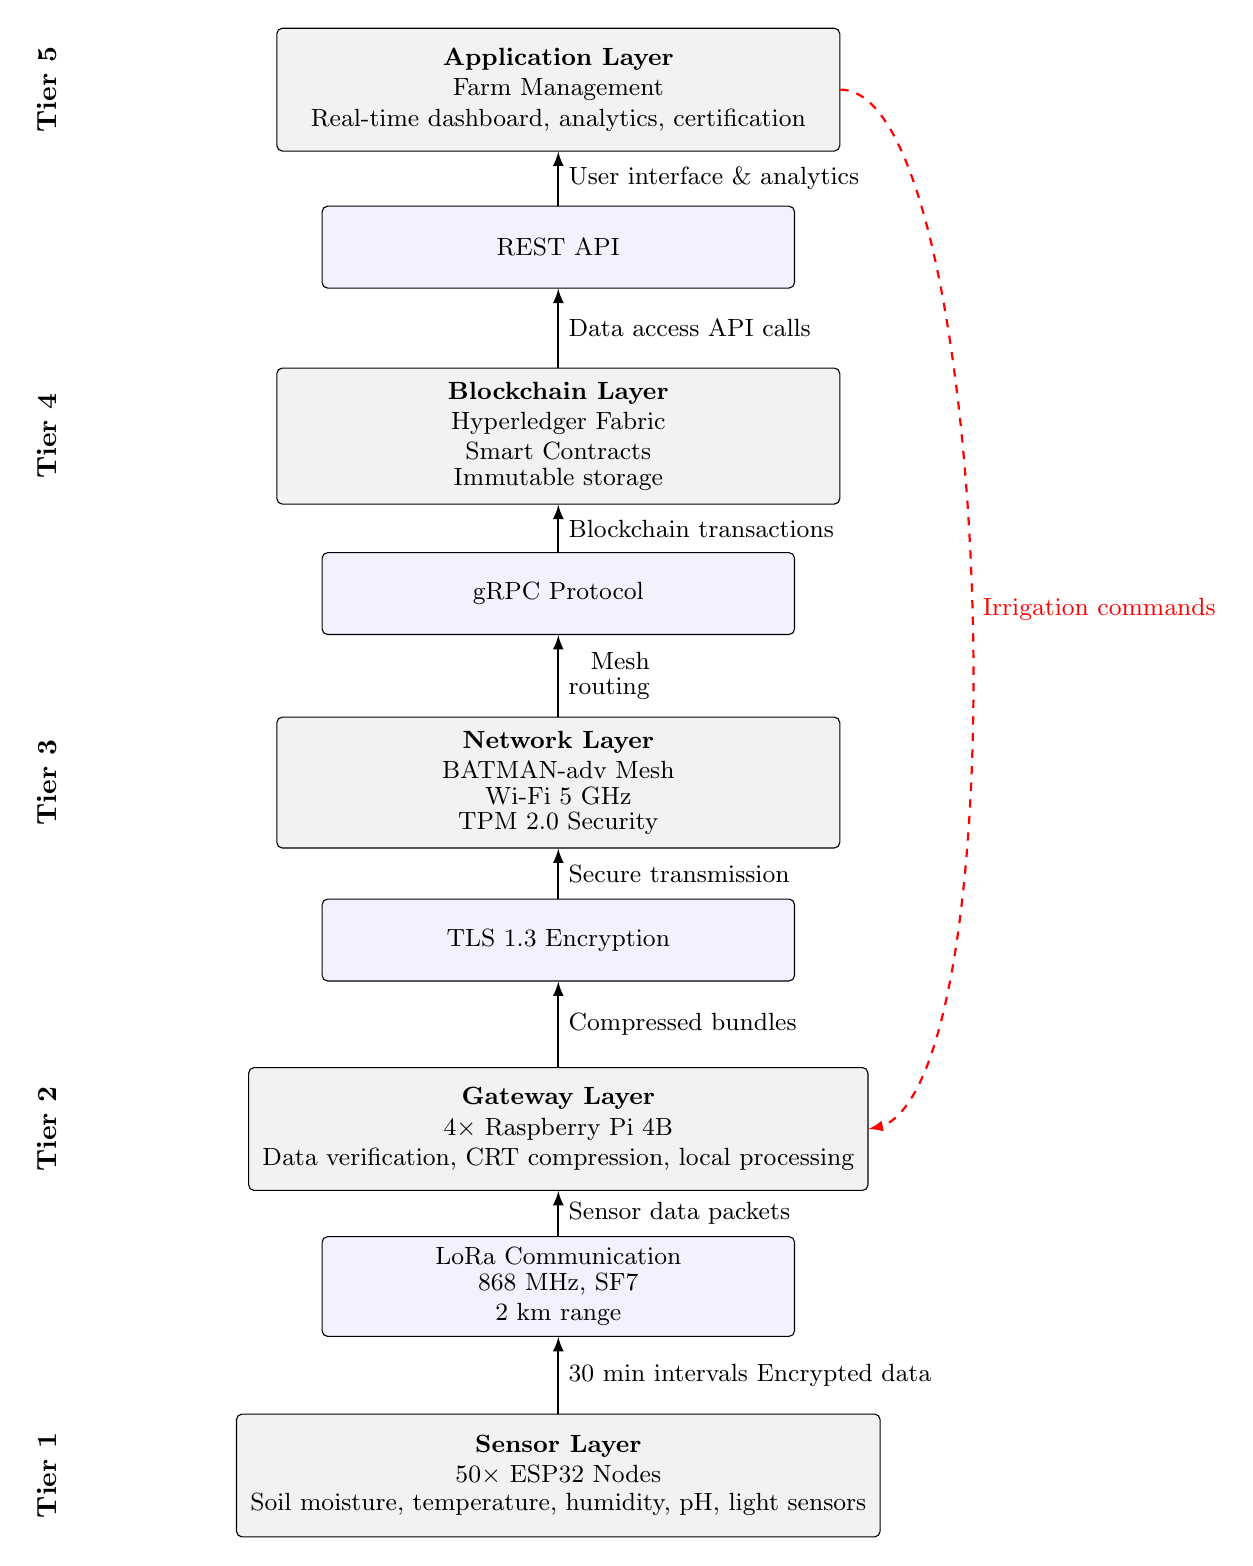
\begin{tikzpicture}[
  font=\small,
  stage/.style={
    draw, rounded corners=2pt, fill=gray!10,
    minimum height=15.6mm,   % 30% taller
    minimum width=71.5mm,    % 30% wider (55mm × 1.3)
    inner sep=5pt
  },
  bluebox/.style={
    draw, rounded corners=2pt, fill=blue!5,
    minimum height=10.4mm,    % 30% taller
    minimum width=60mm,
    inner sep=4pt
  },
  lbl/.style={font=\bfseries, rotate=90},
  >=latex
]

% ---- Tier labels ----
\node[lbl] at (-6.5,10.0) {Tier 5};
\node[lbl] at (-6.5,5.6)  {Tier 4};
\node[lbl] at (-6.5,1.2)  {Tier 3};
\node[lbl] at (-6.5,-3.2) {Tier 2};
\node[lbl] at (-6.5,-7.6) {Tier 1};

% ---- Nodes (4 cm tier gap + 1 cm grey–blue gap) ----
\node[stage] (application) at (0,10.0)
  {\shortstack[c]{\textbf{Application Layer}\\Farm Management\\Real-time dashboard, analytics, certification}};
\node[bluebox] (api) at (0,8.0)
  {\shortstack[c]{REST API}};

\node[stage] (blockchain) at (0,5.6)
  {\shortstack[c]{\textbf{Blockchain Layer}\\Hyperledger Fabric\\Smart Contracts\\Immutable storage}};
\node[bluebox] (grpc) at (0,3.6)
  {\shortstack[c]{gRPC Protocol}};

\node[stage] (mesh) at (0,1.2)
  {\shortstack[c]{\textbf{Network Layer}\\BATMAN-adv Mesh\\Wi-Fi 5 GHz\\TPM 2.0 Security}};
\node[bluebox] (tls) at (0,-0.8)
  {\shortstack[c]{TLS 1.3 Encryption}};

\node[stage] (gateway) at (0,-3.2)
  {\shortstack[c]{\textbf{Gateway Layer}\\4\(\times\) Raspberry Pi 4B\\Data verification, CRT compression, local processing}};
\node[bluebox] (lora) at (0,-5.2)
  {\shortstack[c]{LoRa Communication\\868 MHz, SF7\\2 km range}};

\node[stage] (sensor) at (0,-7.6)
  {\shortstack[c]{\textbf{Sensor Layer}\\50\(\times\) ESP32 Nodes\\Soil moisture, temperature, humidity, pH, light sensors}};

% ---- Arrows ----
\draw[->,thick] (sensor)--node[right]{\shortstack[r]{30 min intervals Encrypted data}}(lora);
\draw[->,thick] (lora)--node[right]{\shortstack[r]{Sensor data packets}}(gateway);
\draw[->,thick] (gateway)--node[right]{\shortstack[r]{Compressed bundles}}(tls);
\draw[->,thick] (tls)--node[right]{\shortstack[r]{Secure transmission}}(mesh);
\draw[->,thick] (mesh)--node[right]{\shortstack[r]{Mesh\\routing}}(grpc);
\draw[->,thick] (grpc)--node[right]{\shortstack[r]{Blockchain transactions}}(blockchain);
\draw[->,thick] (blockchain)--node[right]{\shortstack[r]{Data access API calls}}(api);
\draw[->,thick] (api)--node[right]{\shortstack[r]{User interface \& analytics}}(application);

% ---- Feedback loop ----
\draw[->,thick,red,dashed]
  (application.east)..controls++(2,0)and++(2,0)..
  node[right]{Irrigation commands}(gateway.east);

\end{tikzpicture}
\caption{Five-tier blockchain--IoT architecture with layered tiers and vertical data flow from sensor to application, including a feedback path for irrigation control.}
\label{fig:system-architecture-vertical}
\end{figure}




\subsection{Farm Layout and Network Topology}
\label{subsec:farm_layout}

The system was deployed across a 2-hectare experimental farm (200m × 100m) organized into four operational zones (North, South, East, West). Figure \ref{fig:farm-layout} illustrates the detailed farm layout with sensor placement and communication pathways.

\begin{figure}[!ht]
\centering
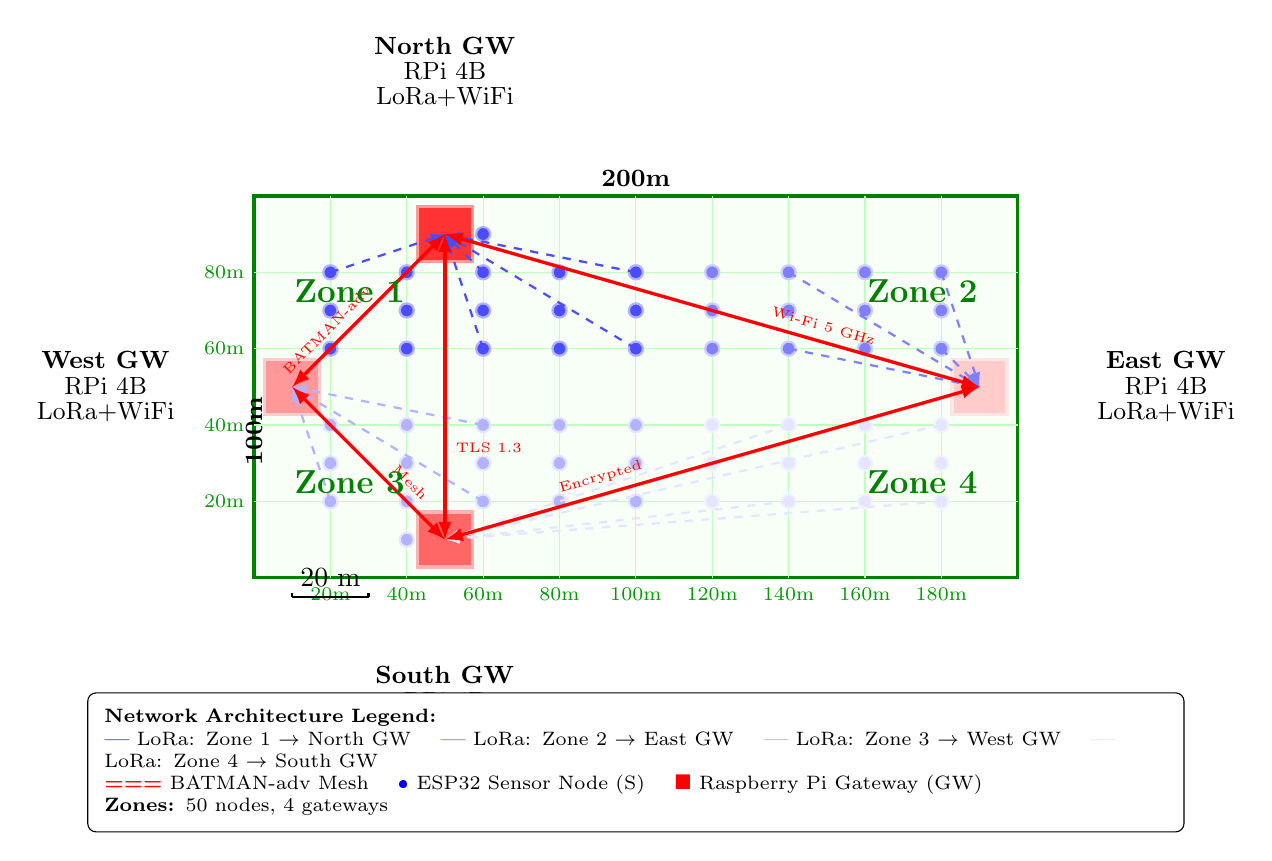
\begin{tikzpicture}[x=0.04\textwidth, y=0.04\textwidth]

% ---------------- FARM DIAGRAM ----------------
\draw[very thick, green!50!black, fill=green!3] (0,0) rectangle (20,10);
\node[above, font=\small\bfseries] at (10,10) {200m};
\node[left, rotate=90, font=\small\bfseries] at (0,5) {100m};

% Grid
\foreach \x in {2,4,...,18} {
  \draw[green!25, thin] (\x,0) -- (\x,10);
  \node[below, font=\scriptsize, green!60!black] at (\x,0) {\x0m};
}
\foreach \y in {2,4,...,8} {
  \draw[green!25, thin] (0,\y) -- (20,\y);
  \node[left, font=\scriptsize, green!60!black] at (0,\y) {\y0m};
}

% Sensors
\foreach \x in {2,4,6,8,10} {
  \foreach \y in {6,7,8} {
    \node[circle, fill=blue!70, draw=blue!30, thick, inner sep=1.8pt,
          label={[font=\tiny, blue!70]center:S}] at (\x,\y) {};
  }
}
\node[circle, fill=blue!70, draw=blue!30, thick, inner sep=1.8pt,
      label={[font=\tiny, blue!70]center:S}] at (6,9) {};

\foreach \x in {12,14,16,18} {
  \foreach \y in {6,7,8} {
    \node[circle, fill=blue!50, draw=blue!20, thick, inner sep=1.8pt,
          label={[font=\tiny, blue!50]center:S}] at (\x,\y) {};
  }
}
\foreach \x in {2,4,6,8,10} {
  \foreach \y in {2,3,4} {
    \node[circle, fill=blue!30, draw=blue!10, thick, inner sep=1.8pt,
          label={[font=\tiny, blue!30]center:S}] at (\x,\y) {};
  }
}
\node[circle, fill=blue!30, draw=blue!10, thick, inner sep=1.8pt,
      label={[font=\tiny, blue!30]center:S}] at (4,1) {};
\foreach \x in {12,14,16,18} {
  \foreach \y in {2,3,4} {
    \node[circle, fill=blue!10, draw=blue!5, thick, inner sep=1.8pt,
          label={[font=\tiny, blue!10]center:S}] at (\x,\y) {};
  }
}

% ---------------- GATEWAYS WITH LABEL SHIFTS ----------------
\node[rectangle, fill=red!80, draw=red!40, very thick, minimum size=7mm,
      label={[font=\small, align=center, yshift=3cm]below:{\shortstack{\textbf{North GW}\\RPi 4B\\LoRa+WiFi}}}] 
      at (5,9) {}; % North shifted upward by 3cm

\node[rectangle, fill=red!60, draw=red!30, very thick, minimum size=7mm,
      label={[font=\small, align=center, yshift=-3cm]above:{\shortstack{\textbf{South GW}\\RPi 4B\\LoRa+WiFi}}}] 
      at (5,1) {}; % South shifted downward by 3cm

\node[rectangle, fill=red!40, draw=red!20, very thick, minimum size=7mm,
      label={[font=\small, align=center, xshift=-1cm]left:{\shortstack{\textbf{West GW}\\RPi 4B\\LoRa+WiFi}}}] 
      at (1,5) {}; % West shifted left by 2cm

\node[rectangle, fill=red!20, draw=red!10, very thick, minimum size=7mm,
      label={[font=\small, align=center, xshift=1cm]right:{\shortstack{\textbf{East GW}\\RPi 4B\\LoRa+WiFi}}}] 
      at (19,5) {}; % East shifted right by 1cm

% LoRa links
\foreach \x in {2,6,10} {
  \foreach \y in {6,8} { \draw[blue!70, dashed, thick, ->] (\x,\y) -- (5,9); }
}
\foreach \x in {14,18} {
  \foreach \y in {6,8} { \draw[blue!50, dashed, thick, ->] (\x,\y) -- (19,5); }
}
\foreach \x in {2,6} {
  \foreach \y in {2,4} { \draw[blue!30, dashed, thick, ->] (\x,\y) -- (1,5); }
}
\foreach \x in {14,18} {
  \foreach \y in {2,4} { \draw[blue!10, dashed, thick, ->] (\x,\y) -- (5,1); }
}

% Mesh backbone
\draw[red, very thick, <->] (5,9) -- node[above, sloped, font=\tiny, pos=0.7] {BATMAN-adv} (1,5);
\draw[red, very thick, <->] (5,9) -- node[above, sloped, font=\tiny, pos=0.7] {Wi-Fi 5 GHz} (19,5);
\draw[red, very thick, <->] (5,9) -- node[right, font=\tiny, pos=0.7] {TLS 1.3} (5,1);
\draw[red, very thick, <->] (1,5) -- node[above, sloped, font=\tiny, pos=0.7] {Mesh} (5,1);
\draw[red, very thick, <->] (19,5) -- node[above, sloped, font=\tiny, pos=0.7] {Encrypted} (5,1);

% Zone labels
\node[font=\large\bfseries, green!50!black] at (2.5,7.5) {Zone 1};
\node[font=\large\bfseries, green!50!black] at (17.5,7.5) {Zone 2};
\node[font=\large\bfseries, green!50!black] at (2.5,2.5) {Zone 3};
\node[font=\large\bfseries, green!50!black] at (17.5,2.5) {Zone 4};

% Scale bar (just below farm)
\draw[thick] (1,-0.5) -- (3,-0.5) node[midway, above] {20 m};
\draw[thick] (1,-0.5) -- (1,-0.4);
\draw[thick] (3,-0.5) -- (3,-0.4);

% ---------------- LEGEND BELOW (shifted down by 1cm) ----------------
\node[
  draw=black, fill=white, rounded corners=3pt, inner sep=6pt,
  font=\scriptsize, text width=13.5cm, align=left,
  anchor=north
] at (10,-3.0) {%
  \textbf{Network Architecture Legend:}\par
  \textcolor{blue!70}{\textbf{---}} LoRa: Zone 1 $\rightarrow$ North GW \quad
  \textcolor{blue!50}{\textbf{---}} LoRa: Zone 2 $\rightarrow$ East GW \quad
  \textcolor{blue!30}{\textbf{---}} LoRa: Zone 3 $\rightarrow$ West GW \quad
  \textcolor{blue!10}{\textbf{---}} LoRa: Zone 4 $\rightarrow$ South GW\par
  \textcolor{red}{\textbf{===}} BATMAN-adv Mesh \quad
  \textcolor{blue}{\textbullet} ESP32 Sensor Node (S) \quad
  {\color{red}\(\blacksquare\)} Raspberry Pi Gateway (GW)\par
  \textbf{Zones:} 50 nodes, 4 gateways%
};

% Extend bounding box further down to prevent overlap with caption
\path (0,-4.6); % invisible depth marker (was -3.6)

\end{tikzpicture}
\caption{Detailed farm network architecture showing 50 ESP32 sensor nodes across four zones, each managed by Raspberry Pi 4B gateways with LoRa communications and a BATMAN-adv mesh backbone for reliable aggregation.}
\label{fig:enhanced-farm-layout}
\end{figure}




Each zone contained 12–13 sensor nodes arranged in a grid pattern with approximately 20-meter spacing, ensuring comprehensive coverage while minimizing communication interference. The gateway placement was optimized for line-of-sight communication with all nodes in their respective zones.

\subsection{Hardware Design and Implementation}
\label{subsec:hardware}

\subsubsection{Sensor Node Architecture}
Each sensor node employed an ESP32-WROOM-32 microcontroller chosen for its dual-core 240 MHz processor, low power consumption (10 $\mu$A in deep sleep), and integrated Wi-Fi/Bluetooth capabilities.


\begin{landscape}
\begin{figure}[p]
\centering

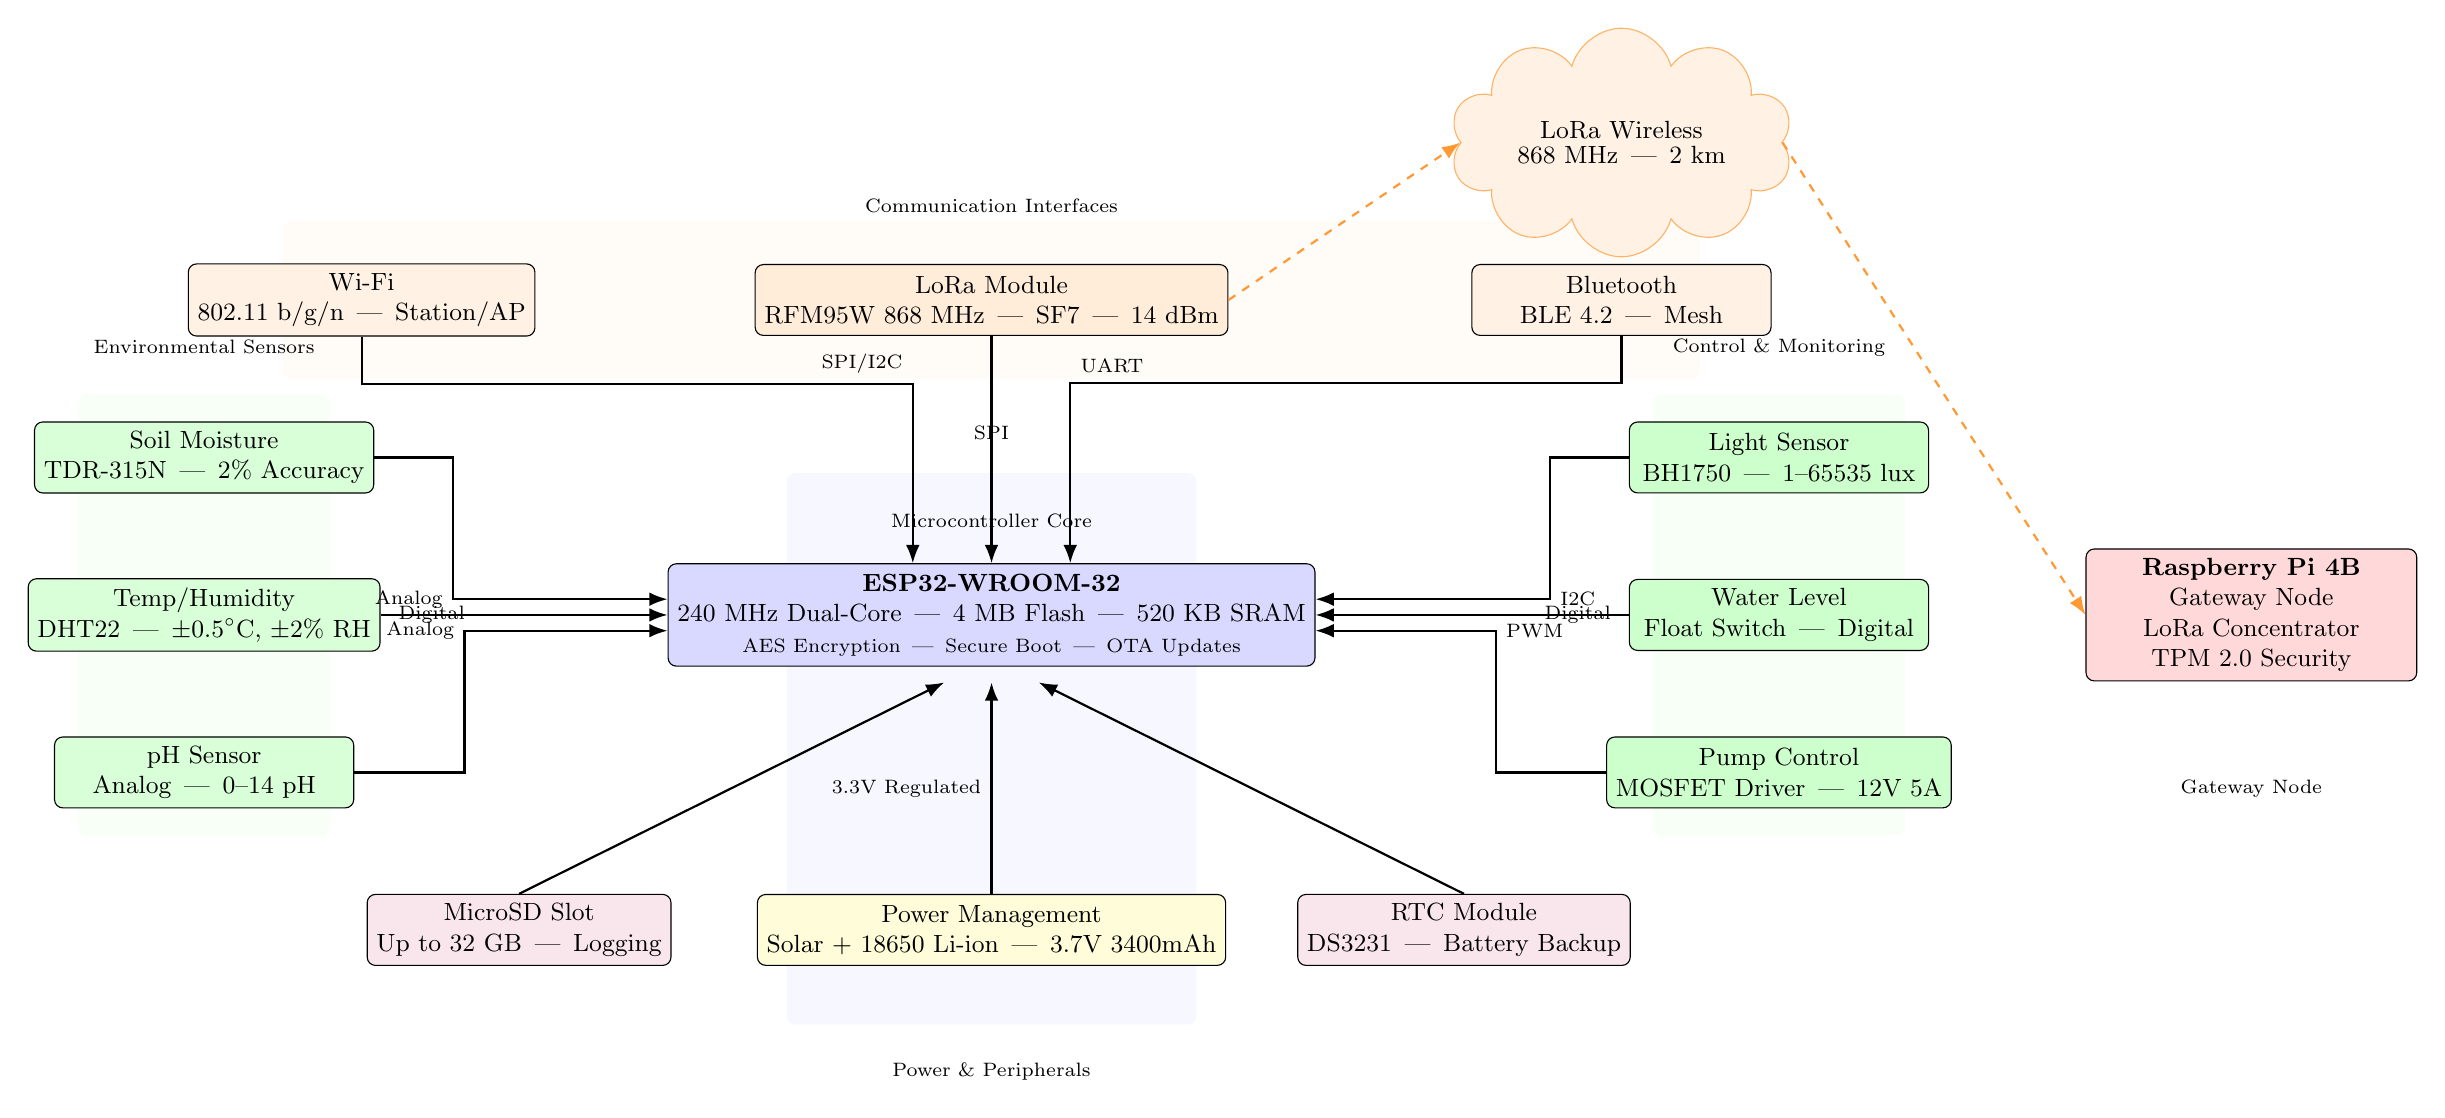
\begin{tikzpicture}[
  font=\small,
  >=Latex,
  % COMPONENT STYLES
  comp/.style={
    draw, rectangle, rounded corners=3pt, minimum width=38mm, minimum height=9mm, align=center, fill=#1
  },
  comp/.default=gray!10,
  arrow/.style={->, thick},
  note/.style={font=\scriptsize, midway}
]

% =================== FIXED COORDINATE LAYOUT ===================
% Main MCU (center)
\node[comp=blue!15, minimum width=45mm, minimum height=13mm] (esp32) at (0,0) {%
  \textbf{ESP32-WROOM-32}\\
  240 MHz Dual-Core \,|\, 4 MB Flash \,|\, 520 KB SRAM\\
  \scriptsize AES Encryption \,|\, Secure Boot \,|\, OTA Updates
};

% COMMUNICATION (top row)
\node[comp=orange!10] (wifi) at (-8,4) {Wi-Fi\\802.11 b/g/n \,|\, Station/AP};
\node[comp=orange!15] (lora) at (0,4) {LoRa Module\\RFM95W 868 MHz \,|\, SF7 \,|\, 14 dBm};
\node[comp=orange!10] (ble)  at (8,4) {Bluetooth\\BLE 4.2 \,|\, Mesh};

% ENVIRONMENTAL (left column)
\node[comp=green!15] (soil) at (-10, 2) {Soil Moisture\\TDR-315N \,|\, 2\% Accuracy};
\node[comp=green!15] (temp) at (-10, 0) {Temp/Humidity\\DHT22 \,|\, $\pm0.5^{\circ}$C, $\pm2$\% RH};
\node[comp=green!15] (ph)   at (-10,-2) {pH Sensor\\Analog \,|\, 0--14 pH};

% CONTROL / OTHER (right column)
\node[comp=green!20] (light) at (10, 2) {Light Sensor\\BH1750 \,|\, 1--65535 lux};
\node[comp=green!20] (water) at (10, 0) {Water Level\\Float Switch \,|\, Digital};
\node[comp=green!20] (pump)  at (10,-2) {Pump Control\\MOSFET Driver \,|\, 12V 5A};

% POWER & PERIPHERALS (bottom row)
\node[comp=yellow!15, minimum width=42mm] (power) at (0,-4) {Power Management\\Solar + 18650 Li-ion \,|\, 3.7V 3400mAh};
\node[comp=purple!10] (storage) at (-6,-4) {MicroSD Slot\\Up to 32 GB \,|\, Logging};
\node[comp=purple!10] (rtc)     at ( 6,-4) {RTC Module\\DS3231 \,|\, Battery Backup};

% GATEWAY (far right)
\node[comp=red!15, minimum width=42mm, minimum height=16mm] (rpi) at (16,0) {%
  \textbf{Raspberry Pi 4B}\\
  Gateway Node\\LoRa Concentrator\\TPM 2.0 Security
};

% CLOUD between ESP32 and RPi (shifted up by 6cm)
\node[cloud, draw=orange!60, fill=orange!10, cloud puffs=10, aspect=2,
      minimum width=28mm, minimum height=14mm] (loracloud) at (8,6) {%
      \shortstack{LoRa Wireless\\868 MHz \,|\, 2 km}};

% =================== CONNECTIONS (NO OVERLAP) ===================
% Left sensors -> ESP32 (route with small jogs)
\draw[arrow] (soil.east) -- ++(1.0,0) |- ([yshift=2mm] esp32.west) node[note, left] {Analog};
\draw[arrow] (temp.east) -- ++(1.2,0) |- (esp32.west) node[note, left] {Digital};
\draw[arrow] (ph.east)   -- ++(1.4,0) |- ([yshift=-2mm] esp32.west) node[note, left] {Analog};

% Right sensors -> ESP32
\draw[arrow] (light.west) -- ++(-1.0,0) |- ([yshift=2mm] esp32.east) node[note, right] {I2C};
\draw[arrow] (water.west) -- ++(-1.2,0) |- (esp32.east) node[note, right] {Digital};
\draw[arrow] (pump.west)  -- ++(-1.4,0) |- ([yshift=-2mm] esp32.east) node[note, right] {PWM};

% Comms -> ESP32
\draw[arrow] (wifi.south) -- ++(0,-0.6) -| ([xshift=-10mm] esp32.north) node[note, above left] {SPI/I2C};
\draw[arrow] (lora.south) -- (esp32.north) node[note, above] {SPI};
\draw[arrow] (ble.south)  -- ++(0,-0.6) -| ([xshift=10mm] esp32.north)  node[note, above right] {UART};

% Power & peripherals -> ESP32
\draw[arrow] (power.north)   -- ([yshift=-2mm] esp32.south) node[note, left] {3.3V Regulated};
\draw[arrow] (storage.north) -- ([xshift=-6mm,yshift=-2mm] esp32.south);
\draw[arrow] (rtc.north)     -- ([xshift= 6mm,yshift=-2mm] esp32.south);

% LoRa wireless -> RPi via cloud
\draw[arrow, dashed, orange!80] (lora.east) -- (loracloud.west);
\draw[arrow, dashed, orange!80] (loracloud.east) -- (rpi.west);

% =================== SECTION BACKGROUNDS ===================
\begin{scope}[on background layer]
  \fill[blue!3,  rounded corners=3pt] (-2.6,  1.8) rectangle ( 2.6,-5.2);  % MCU + power zone
  \fill[green!3, rounded corners=3pt] (-11.6, 2.8) rectangle (-8.4,-2.8);   % left sensors
  \fill[green!3, rounded corners=3pt] (  8.4,  2.8) rectangle (11.6,-2.8);  % right sensors
  \fill[orange!3,rounded corners=3pt] (-9.0,  5.0) rectangle ( 9.0, 3.0);   % comms
\end{scope}

% Section labels (placed away from connectors)
\node[font=\scriptsize] at (0,  5.2) {Communication Interfaces};
\node[font=\scriptsize] at (0, -5.8) {Power \& Peripherals};
\node[font=\scriptsize] at (-10.0, 3.4) {Environmental Sensors};
\node[font=\scriptsize] at ( 10.0, 3.4) {Control \& Monitoring};
\node[font=\scriptsize] at (16.0, -2.2) {Gateway Node};
\node[font=\scriptsize] at (0,  1.2) {Microcontroller Core};

\end{tikzpicture}

\caption{Enhanced ESP32 sensor node architecture showing clearly separated sensor inputs, communication modules, power/peripheral interfaces, and the LoRa wireless link to a Raspberry Pi~4B gateway for a blockchain–IoT agriculture deployment.}
\label{fig:enhanced-sensor-node}
\end{figure}
\end{landscape}


The nodes incorporated multiple sensors optimized for agricultural monitoring:

\begin{itemize}
    \item \textbf{Soil moisture}: TDR-315N probes measuring volumetric water content with 2\% accuracy
    \item \textbf{Temperature and humidity}: DHT22 sensors with ±0.5°C and ±2\% RH accuracy
    \item \textbf{pH sensors}: Analog sensors with amplifier circuit for soil acidity monitoring
    \item \textbf{Light intensity}: BH1750 sensors for photosynthetic active radiation measurement
    \item \textbf{Water level}: Float switches for irrigation system monitoring
\end{itemize}

Each node included a RFM95W LoRa module for long-range communication (up to 2 km in rural environments) and was powered by 18650 lithium batteries (3400 mAh) charged via 6V 3W solar panels, enabling 34-day operation between charges under normal conditions.

\subsubsection{Gateway Architecture}
Raspberry Pi 4B devices (4GB RAM) served as gateways, providing sufficient processing power for data aggregation, CRT compression, and local decision making. Each gateway managed up to 13 sensor nodes and included:

\begin{itemize}
    \item LoRa concentrator (SX1302) for receiving sensor data from multiple nodes
    \item TPM 2.0 module for secure key storage and cryptographic operations
    \item Dual-band Wi-Fi for mesh networking and backup connectivity
    \item 128 GB microSD card for local storage and buffer during connectivity loss
    \item GPS module for precise timing and location services
\end{itemize}

Figure \ref{fig:gateway-arch} illustrates the gateway architecture and data processing flow.

\begin{landscape}
\begin{figure}[!ht]
\centering
\resizebox{0.95\linewidth}{!}{%
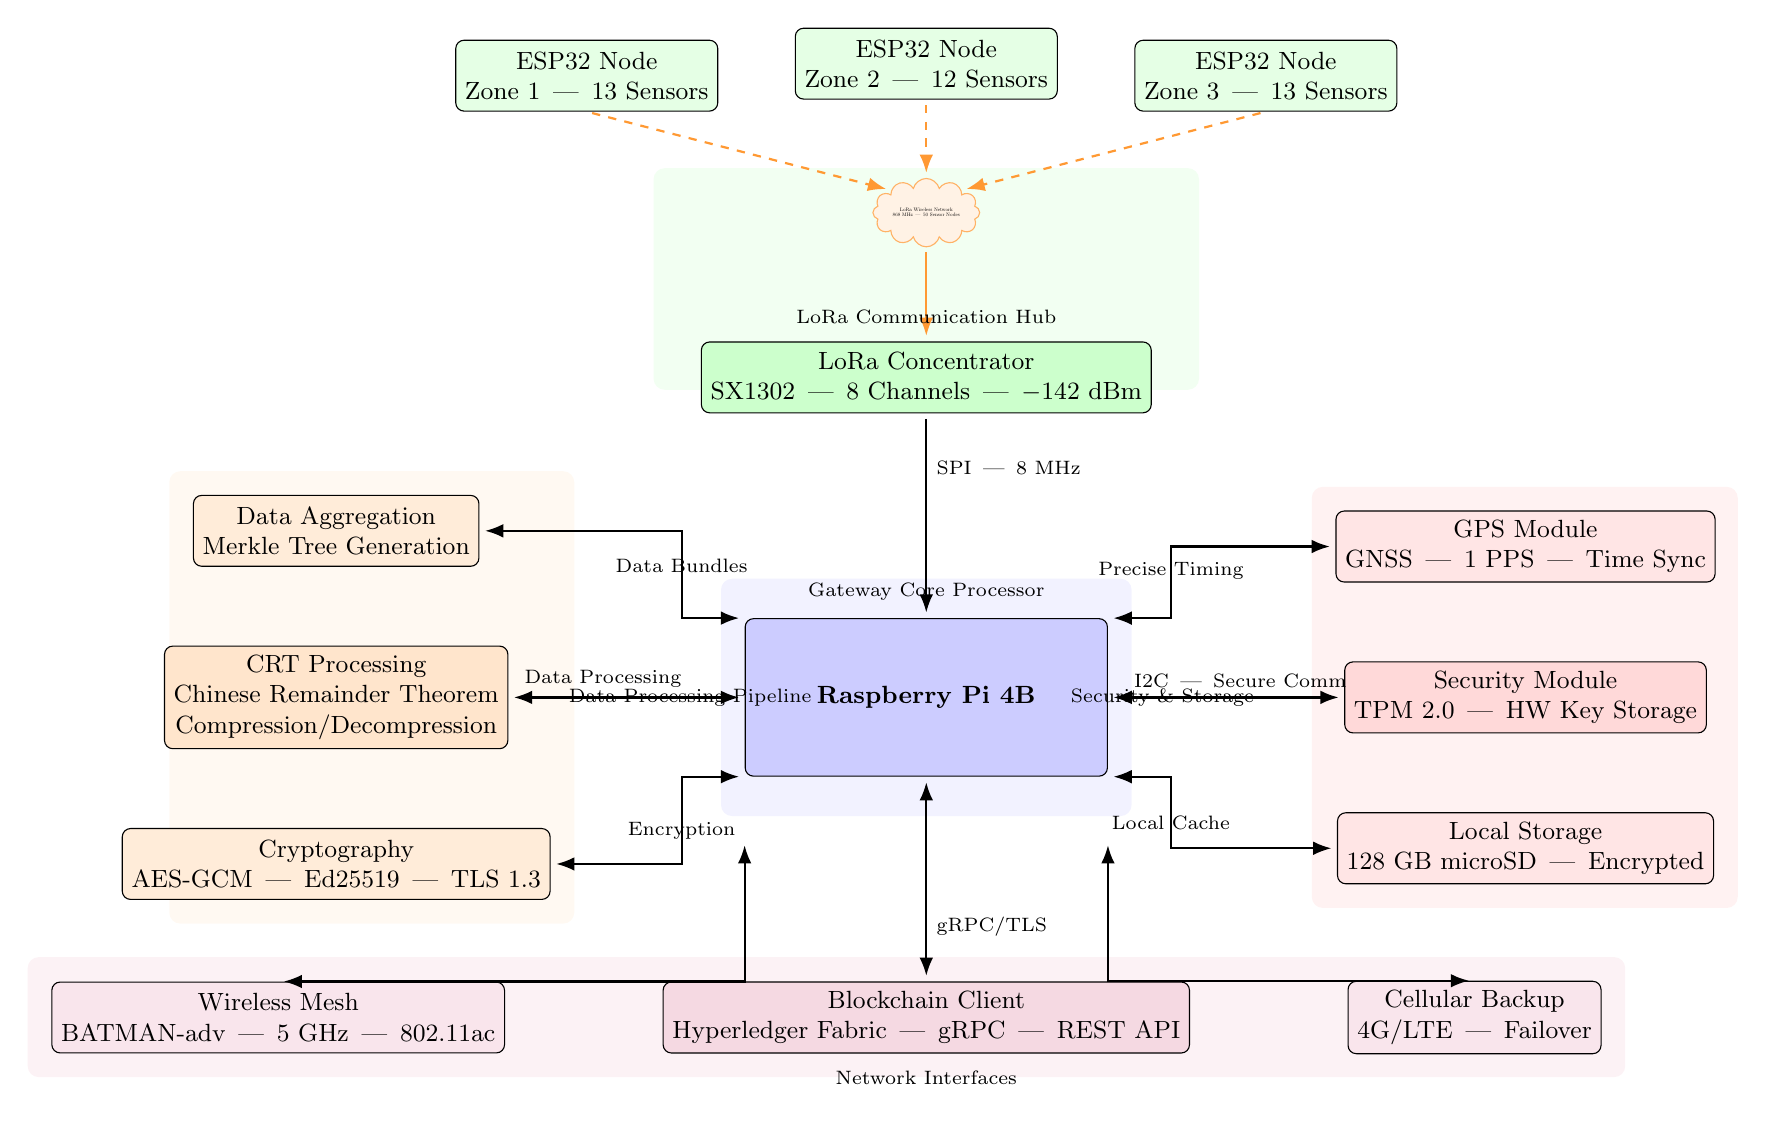
\begin{tikzpicture}[
    >=Latex,
    every node/.style={font=\small},
    component/.style={
        draw, rectangle, rounded corners=3pt, fill=#1,
        minimum width=32mm, minimum height=9mm, align=center
    },
    arrow/.style={-Latex, thick, shorten >=2pt, shorten <=2pt},
    label/.style={font=\scriptsize},
    cloudnode/.style={
      draw=orange!60, fill=orange!10,
      shape=cloud, cloud puffs=12, aspect=2,
      minimum width=30mm, minimum height=14mm
    }
]

% ==================== CORE ====================
\node[component=blue!20, minimum width=46mm, minimum height=20mm] (pi) at (0,0) {\textbf{Raspberry Pi 4B}};

% ==================== LORA STACK (TOP) ====================
\node[component=green!20, above=26mm of pi] (lora) {LoRa Concentrator\\SX1302 \,|\, 8 Channels \,|\, $-142$ dBm};
\node[cloudnode, above=12mm of lora, transform shape, scale=0.2] (loracloud)
  {\shortstack{LoRa Wireless Network\\868 MHz \,|\, 50 Sensor Nodes}};

% ESP32 aggregators
\node[component=green!10, above left=10mm and 22mm of loracloud] (node1) {ESP32 Node\\Zone 1 \,|\, 13 Sensors};
\node[component=green!10, above=10mm of loracloud]                (node2) {ESP32 Node\\Zone 2 \,|\, 12 Sensors};
\node[component=green!10, above right=10mm and 22mm of loracloud] (node3) {ESP32 Node\\Zone 3 \,|\, 13 Sensors};

% ==================== LEFT PROCESSING ====================
\node[component=orange!20, left=30mm of pi] (crt) {CRT Processing\\Chinese Remainder Theorem\\Compression/Decompression};
\node[component=orange!15, above=10mm of crt] (data) {Data Aggregation\\Merkle Tree Generation};
\node[component=orange!15, below=10mm of crt] (crypto) {Cryptography\\AES-GCM \,|\, Ed25519 \,|\, TLS 1.3};

% ==================== RIGHT SECURITY / STORAGE ====================
\node[component=red!15, right=30mm of pi] (tpm) {Security Module\\TPM 2.0 \,|\, HW Key Storage};
\node[component=red!10, above=10mm of tpm] (gps) {GPS Module\\GNSS \,|\, 1 PPS \,|\, Time Sync};
\node[component=red!10, below=10mm of tpm] (storage) {Local Storage\\128 GB microSD \,|\, Encrypted};

% ==================== BOTTOM NETWORK ====================
\node[component=purple!15, below=26mm of pi] (blockchain) {Blockchain Client\\Hyperledger Fabric \,|\, gRPC \,|\, REST API};
\node[component=purple!10, left=20mm of blockchain]  (wifi) {Wireless Mesh\\BATMAN-adv \,|\, 5 GHz \,|\, 802.11ac};
\node[component=purple!10, right=20mm of blockchain] (cellular) {Cellular Backup\\4G/LTE \,|\, Failover};

% ==================== LINKS (ROUTED & LABELED OFF-BOX) ====================

% LoRa fan-in
\draw[arrow, dashed, orange!80] (node1.south) -- (loracloud.north west);
\draw[arrow, dashed, orange!80] (node2.south) -- (loracloud.north);
\draw[arrow, dashed, orange!80] (node3.south) -- (loracloud.north east);
\draw[arrow, thick,  orange!80] (loracloud.south) -- (lora.north);

% Concentrator to Pi (label offset to the side)
\draw[arrow, thick] (lora.south) -- node[label, right, pos=0.3] {SPI \,|\, 8 MHz} ([yshift=3mm]pi.north)
                     -- ([yshift=0mm]pi.north);

% Left side -> Pi (place labels on the horizontal jogs)
\draw[arrow, thick,<->] (data.east)  -| node[label, above, pos=0.8] {Data Bundles} ([xshift=-8mm]pi.north west) -- (pi.north west);
\draw[arrow, thick,<->] (crt.east)   -- node[label, above, pos=0.5] {Data Processing} ([xshift=-6mm]pi.west) -- (pi.west);
\draw[arrow, thick,<->] (crypto.east) -| node[label, below, pos=0.8] {Encryption} ([xshift=-8mm]pi.south west) -- (pi.south west);

% Right side -> Pi (labels kept off the Pi box)
\draw[arrow, thick,<->] (gps.west)    -| node[label, above, pos=0.8] {Precise Timing} ([xshift=8mm]pi.north east) -- (pi.north east);
\draw[arrow, thick,<->] (tpm.west)     -- node[label, above, pos=0.55] {I2C \,|\, Secure Comm} ([xshift=6mm]pi.east) -- (pi.east);
\draw[arrow, thick,<->] (storage.west) -| node[label, below, pos=0.8] {Local Cache} ([xshift=8mm]pi.south east) -- (pi.south east);

% Bottom -> Pi
\draw[arrow, thick,<->] (blockchain.north) -- node[label, right, pos=0.3] {gRPC/TLS} ([yshift=-3mm]pi.south) -- (pi.south);
\draw[arrow, thick,<->] (wifi.north)      -| ([yshift=-8mm]pi.south west);
\draw[arrow, thick,<->] (cellular.north)  -| ([yshift=-8mm]pi.south east);

% Cloud → concentrator arrows already above

% ==================== BACKGROUND BANDS ====================
\begin{scope}[on background layer]
  \fill[blue!5,   rounded corners]
       ($(pi.north west)+(-3mm,5mm)$) rectangle ($(pi.south east)+(3mm,-5mm)$);
  \fill[green!5,  rounded corners]
       ($(lora.north west)+(-6mm,22mm)$) rectangle ($(lora.south east)+(6mm,3mm)$);
  \fill[orange!5, rounded corners]
       ($(data.north west)+(-3mm,3mm)$) rectangle ($(crypto.south east)+(3mm,-3mm)$);
  \fill[red!5,    rounded corners]
       ($(gps.north west)+(-3mm,3mm)$) rectangle ($(storage.south east)+(3mm,-3mm)$);
  \fill[purple!5, rounded corners]
       ($(wifi.south west)+(-3mm,-3mm)$) rectangle ($(cellular.north east)+(3mm,3mm)$);
\end{scope}

% ==================== SECTION LABELS ====================
\node[font=\scriptsize, above=1mm of lora] {LoRa Communication Hub};
\node[font=\scriptsize, above=1mm of pi]   {Gateway Core Processor};
\node[font=\scriptsize] at (-30mm,  0mm)   {Data Processing Pipeline};
\node[font=\scriptsize] at ( 30mm,  0mm)   {Security \& Storage};
\node[font=\scriptsize, below=1mm of blockchain] {Network Interfaces};

\end{tikzpicture}
}
\caption{Enhanced Raspberry Pi 4B gateway architecture with clean routing and labeling.}
\label{fig:enhanced-gateway-arch}
\end{figure}
\end{landscape}



\subsection{Node Communication Protocol}
\label{subsec:communication_protocol}

\subsubsection{LoRa Communication Framework}
The sensor nodes communicated with gateways using LoRaWAN protocol in the 868 MHz band with the following parameters:

\begin{table}[!ht]
\centering
\caption{LoRa communication parameters for node-gateway communication}
\label{tab:lora-params}
\begin{tabular}{lcc}
\toprule
\textbf{Parameter} & \textbf{Value} & \textbf{Description} \\
\midrule
Frequency & 868.1 MHz & EU ISM band \\
Spreading Factor & SF7 & Balance range and airtime \\
Bandwidth & 125 kHz & Standard LoRa bandwidth \\
Coding Rate & 4/5 & Error correction rate \\
Transmit Power & 14 dBm & Maximum allowed power \\
Sensitivity & -137 dBm & Receiver sensitivity \\
Data Rate & 5.47 kbps & Effective data rate \\
Airtime (32B) & 247 ms & Time-on-air per packet \\
Airtime (8B) & 124 ms & CRT compressed packet \\
\bottomrule
\end{tabular}
\end{table}

The communication followed a hybrid polling and event-driven approach:

\begin{itemize}
    \item \textbf{Periodic Polling}: Gateways polled each node in assigned TDMA slots every 30 minutes
    \item \textbf{Event-Driven Alerts}: Nodes immediately transmitted data when thresholds were breached
    \item \textbf{Acknowledgment Protocol}: Two-way communication ensured data reliability
\end{itemize}

\subsubsection{Data Frame Structure}
The sensor data was structured in optimized frames for efficient transmission:

\begin{table}[!ht]
\centering
\caption{Data frame structure for sensor node communication}
\label{tab:data-frame}
\begin{tabular}{lccc}
\toprule
\textbf{Field} & \textbf{Size (bytes)} & \textbf{CRT Compressed} & \textbf{Description} \\
\midrule
Node ID & 2 & 2 & Unique sensor identifier \\
Timestamp & 4 & 4 & Unix timestamp \\
Soil Moisture & 4 & 2 & Volumetric water content \\
Temperature & 4 & 2 & Celsius × 100 \\
Humidity & 4 & 2 & Relative humidity × 100 \\
pH Value & 4 & 2 & pH × 100 \\
Light Intensity & 4 & 2 & Lux measurement \\
Battery Level & 1 & 1 & Percentage (0-100) \\
Signature & 32 & 32 & Ed25519 signature \\
\hline
\textbf{Total Size} & \textbf{59 bytes} & \textbf{47 bytes} & \textbf{20\% reduction} \\
\bottomrule
\end{tabular}
\end{table}

\subsubsection{Mesh Network Communication}
Gateways communicated with each other and the central server using BATMAN-adv (Better Approach To Mobile Adhoc Networking) mesh protocol over 5 GHz Wi-Fi. This provided:

\begin{itemize}
    \item Self-healing network topology
    \item Automatic route optimization
    \item Load balancing across multiple paths
    \item Fault tolerance for gateway failures
\end{itemize}

The mesh network maintained an average latency of 15–25 ms between gateways with 99.8\% packet delivery rate during normal operation.

\subsection{Chinese Remainder Theorem Data Compression}
\label{subsec:crt_compression}

\subsubsection{Mathematical Foundation}
The Chinese Remainder Theorem provides a method for representing large integers using smaller residues. Given pairwise coprime moduli $m_1, m_2, \ldots, m_k$, any integer $x$ in the range $[0, M)$ where $M = \prod_{i=1}^k m_i$ can be uniquely represented by its residues:
\[
r_i = x \mod m_i \quad \text{for } i = 1, 2, \ldots, k
\]
The original value can be reconstructed using Garner's algorithm:
\[
x = \left( \sum_{i=1}^k r_i \cdot M_i \cdot (M_i^{-1} \mod m_i) \right) \mod M
\]
where $M_i = M / m_i$.

\subsubsection{Agricultural Data Application}
For agricultural sensor data, we applied CRT compression as follows:

\begin{enumerate}
    \item Sensor readings were scaled to integers (e.g., temperature 25.3°C became 2530)
    \item Scaled values were decomposed into residues using selected moduli sets
    \item Residues were transmitted instead of full 32-bit values
    \item Gateways reconstructed original values using CRT with Garner's algorithm
\end{enumerate}

We implemented three moduli sets optimized for different precision requirements:

\begin{table}[!ht]
\centering
\caption{CRT moduli sets for different precision requirements}
\label{tab:crt-moduli}
\begin{tabular}{lccc}
\toprule
\textbf{Parameter} & \textbf{Basic Precision} & \textbf{Standard Precision} & \textbf{High Precision} \\
\midrule
Moduli Set & [97, 101] & [97, 101, 103] & [97, 101, 103, 107] \\
Residues per value & 2 & 3 & 4 \\
Bytes per value & 2 & 3 & 4 \\
Maximum Value & 9,797 & 1,009,091 & 107,972,791 \\
Compression Ratio & 50\% & 25\% & 0\% \\
Application & Temperature & Soil moisture & High-precision pH \\
Reconstruction Error & 0\% & 0\% & 0\% \\
\bottomrule
\end{tabular}
\end{table}

\subsubsection{Compression Performance}
The CRT compression achieved significant efficiency improvements:

\begin{table}[!ht]
\centering
\caption{CRT compression performance across different data types}
\label{tab:crt-performance}
\begin{tabular}{lcccc}
\toprule
\textbf{Data Type} & \textbf{Original Size} & \textbf{CRT Compressed} & \textbf{Reduction} & \textbf{Processing Time} \\
\midrule
Temperature & 4 bytes & 2 bytes & 50\% & 0.8 ms \\
Soil Moisture & 4 bytes & 3 bytes & 25\% & 1.2 ms \\
Humidity & 4 bytes & 2 bytes & 50\% & 0.7 ms \\
pH Value & 4 bytes & 3 bytes & 25\% & 1.1 ms \\
Light Intensity & 4 bytes & 2 bytes & 50\% & 0.9 ms \\
\hline
\textbf{Average} & \textbf{4 bytes} & \textbf{2.4 bytes} & \textbf{40\%} & \textbf{0.94 ms} \\
\bottomrule
\end{tabular}
\end{table}

\subsection{Blockchain Implementation}
\label{subsec:blockchain}

We implemented a permissioned blockchain using Hyperledger Fabric 2.4, chosen for its modular architecture and support for smart contracts. Key design decisions:

\begin{itemize}
    \item \textbf{Consensus}: Raft ordering service for efficient consensus in trusted environments
    \item \textbf{Smart Contracts}: Chaincode for sensor registration, data validation, and irrigation rules
    \item \textbf{Data Storage}: On-chain storage of cryptographic hashes with off-chain storage of detailed sensor data
    \item \textbf{Access Control}: Role-based permissions for farmers, agronomists, and certification bodies
\end{itemize}

The blockchain network consisted of:
\begin{itemize}
    \item 3 Orderer nodes running Raft consensus
    \item 4 Peer nodes (one per gateway zone)
    \item 1 Certificate Authority for identity management
    \item 1 CouchDB instance for state database
\end{itemize}

\section{Materials and Methods}
\label{sec:materials_methods}

\subsection{Study Site and Environmental Conditions}
\label{subsec:study_site}

The field study was conducted in Sfax, Tunisia (34.74°N, 10.76°E) during August and September 2024. Sfax experiences a Mediterranean climate with hot, dry summers. Detailed environmental conditions during the study period:

\begin{table}[!ht]
\centering
\caption{Environmental conditions during study period (August-September 2024)}
\label{tab:environmental}
\begin{tabular}{lccc}
\toprule
\textbf{Parameter} & \textbf{August} & \textbf{September} & \textbf{Source} \\
\midrule
Average Temperature & 31.5°C & 28.8°C & On-site monitoring \\
Maximum Temperature & 38.2°C & 34.7°C & On-site monitoring \\
Minimum Temperature & 23.4°C & 21.2°C & On-site monitoring \\
Relative Humidity & 58\% & 63\% & On-site monitoring \\
Rainfall & 8.2 mm & 14.7 mm & Tunisia Meteorological Institute \\
Solar Radiation & 7.8 kWh/m²/day & 6.9 kWh/m²/day & On-site monitoring \\
Wind Speed & 3.2 m/s & 2.8 m/s & On-site monitoring \\
\bottomrule
\end{tabular}
\end{table}

Soil characteristics at the study site:
\begin{itemize}
    \item \textbf{Texture}: Sandy loam (62\% sand, 28\% silt, 10\% clay)
    \item \textbf{pH}: 6.8 (slightly acidic)
    \item \textbf{Organic matter}: 1.5\% 
    \item \textbf{Bulk density}: 1.35 g/cm³
    \item \textbf{Field capacity}: 28\% volumetric
    \item \textbf{Wilting point}: 12\% volumetric
\end{itemize}

\subsection{Crop Management Practices}
\label{subsec:crop_management}

\subsubsection{Tomato Cultivation (\textit{Solanum lycopersicum})}
\begin{itemize}
    \item \textbf{Variety}: Rio Grande (determinate processing type) and hybrid salad types
    \item \textbf{Nursery}: Late May to mid-June sowing, 4–6 week seedling period
    \item \textbf{Transplanting}: Late June to early July at 5–7 true leaf stage
    \item \textbf{Spacing}: 1.0–1.2 m between rows, 35–50 cm in-row (16,000–28,000 plants/ha)
    \item \textbf{Support}: Staking and pruning of indeterminate varieties
    \item \textbf{Fertilization}: Basal application + fertigation (N 150-200 kg/ha, P₂O₅ 80-120 kg/ha, K₂O 200-300 kg/ha)
    \item \textbf{Harvest}: First pick mid-August to September, main harvest through October
\end{itemize}

\subsubsection{Pepper Cultivation (\textit{Capsicum spp.})}
\begin{itemize}
    \item \textbf{Varieties}: Baklouti chili and bell pepper types
    \item \textbf{Nursery}: Early to mid-May sowing, 6–8 week seedling period
    \item \textbf{Transplanting}: Late June to early July
    \item \textbf{Spacing}: 0.6–0.8 m between rows, 30–40 cm in-row (31,000–55,000 plants/ha)
    \item \textbf{Support}: Staking against late summer winds
    \item \textbf{Fertilization}: Basal application + fertigation (N 120-180 kg/ha, P₂O₅ 60-100 kg/ha, K₂O 150-250 kg/ha)
    \item \textbf{Harvest}: First pick late August to September, continuing through October
\end{itemize}

\subsection{Experimental Design}
\label{subsec:experimental_design}

The study employed a randomized complete block design with three replications for each treatment:

\begin{itemize}
    \item \textbf{Treatment 1}: Blockchain-IoT system with CRT compression and automated irrigation
    \item \textbf{Treatment 2}: Traditional irrigation practices based on visual assessment (control)
    \item \textbf{Plot sizes}: Tomatoes 0.5 ha, Peppers 0.3 ha per treatment
    \item \textbf{Replications}: 3 blocks per treatment, randomized within blocks
\end{itemize}

Both treatments used identical drip irrigation systems with pressure-compensating emitters (2.0 L/h flow rate) to ensure comparable water application efficiency. The traditional practice followed conventional scheduling based on visual assessment and fixed timers, while the blockchain-IoT system used soil moisture-based automation with the following thresholds:

\begin{table}[!ht]
\centering
\caption{Irrigation thresholds for blockchain-IoT system}
\label{tab:irrigation-thresholds}
\begin{tabular}{lccc}
\toprule
\textbf{Crop} & \textbf{Growth Stage} & \textbf{Soil Moisture Threshold} & \textbf{Irrigation Duration} \\
\midrule
Tomato & Vegetative & -35 kPa & 30 minutes \\
Tomato & Flowering & -30 kPa & 40 minutes \\
Tomato & Fruit Development & -25 kPa & 45 minutes \\
Tomato & Ripening & -35 kPa & 30 minutes \\
Pepper & Vegetative & -30 kPa & 25 minutes \\
Pepper & Flowering & -25 kPa & 35 minutes \\
Pepper & Fruit Development & -20 kPa & 40 minutes \\
Pepper & Maturation & -30 kPa & 30 minutes \\
\bottomrule
\end{tabular}
\end{table}

\subsection{Data Collection and Analysis}
\label{subsec:data_collection}

Comprehensive data collection included multiple parameters across technical, agricultural, and economic dimensions:

\begin{itemize}
    \item \textbf{Soil parameters}: Moisture (30-min intervals), temperature, pH
    \item \textbf{Climate data}: Temperature, humidity, solar radiation (hourly)
    \item \textbf{Water use}: Precision flow meters on irrigation lines (0.5\% accuracy)
    \item \textbf{System performance}: Latency, reliability, energy consumption, data accuracy
    \item \textbf{Labor inputs}: Time-motion studies for all farming activities
    \item \textbf{Crop performance}: Yield, fruit quality, water use efficiency
    \item \textbf{Economic data}: Input costs, labor costs, water costs, yield value
\end{itemize}

Statistical analysis was performed using R 4.2.1 with ANOVA and Tukey's HSD test for mean separation at p < 0.05 significance level. Economic analysis included net present value (NPV) and return on investment (ROI) calculations over a 5-year horizon.

\section{Results and Discussion}
\label{sec:results}

\subsection{System Performance Metrics}
\label{subsec:system_performance}

The blockchain-IoT system demonstrated robust performance across all measured parameters during the 61-day study period:

\begin{table}[!ht]
\centering
\caption{Comprehensive system performance metrics (August-September 2024)}
\label{tab:system-performance}
\begin{tabular}{lccc}
\toprule
\textbf{Performance Metric} & \textbf{Target} & \textbf{Achieved} & \textbf{Variation} \\
\midrule
Data Reliability & 99.0\% & 99.4\% & +0.4\% \\
Average Latency & <2.0 s & 1.7 s & -0.3 s \\
P95 Latency & <3.0 s & 2.4 s & -0.6 s \\
P99 Latency & <5.0 s & 3.8 s & -1.2 s \\
Data Accuracy & 98.0\% & 99.1\% & +1.1\% \\
Battery Life & 30 days & 34 days & +4 days \\
Network Uptime & 99.0\% & 99.6\% & +0.6\% \\
CRT Compression & 30\% & 33\% & +3\% \\
Energy Consumption & <100 Wh/day & 87 Wh/day & -13\% \\
Data Storage & <2 GB & 1.4 GB & -0.6 GB \\
\bottomrule
\end{tabular}
\end{table}

Figure \ref{fig:system-metrics} illustrates the key performance metrics throughout the study period, showing consistent operation with minor variations due to environmental conditions.

\begin{figure}[!ht]
\centering
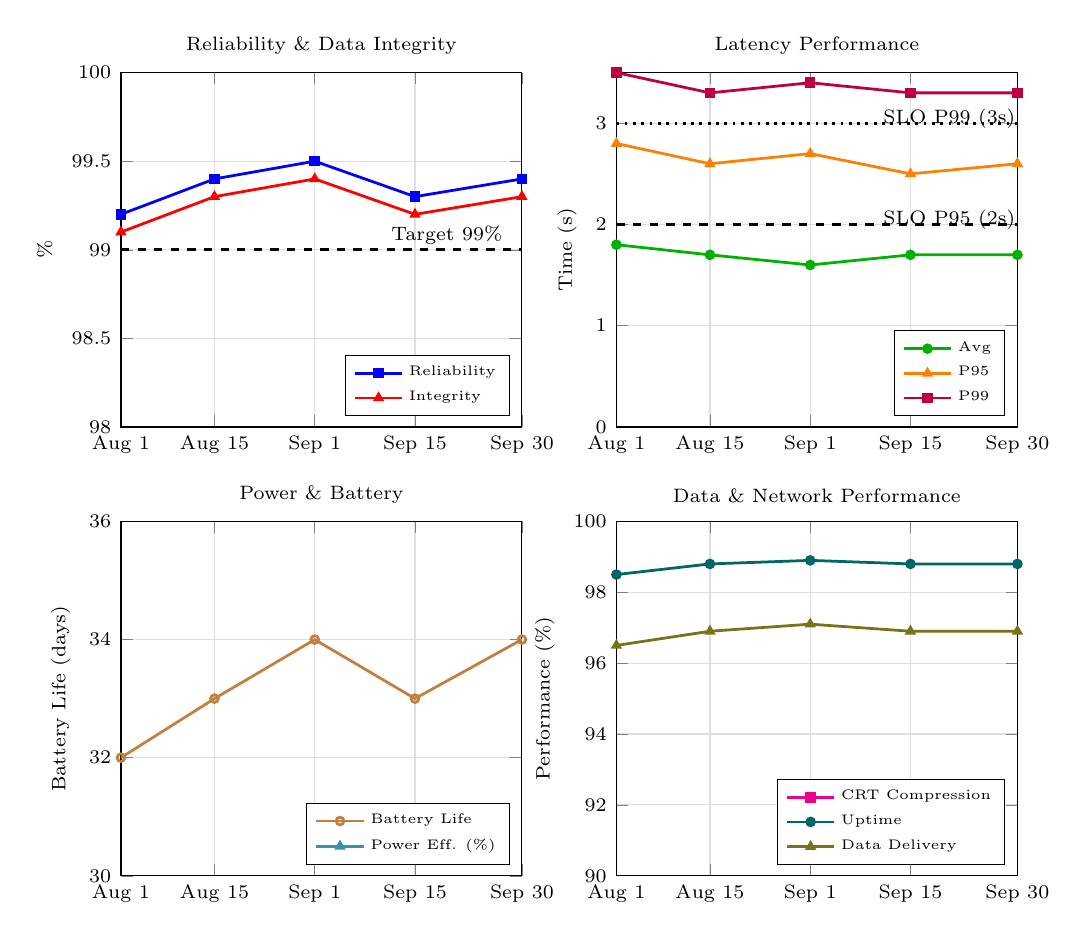
\begin{tikzpicture}
\begin{groupplot}[
  group style={
    group size=2 by 2,
    horizontal sep=1.2cm,
    vertical sep=1.2cm
  },
  width=0.42\textwidth,
  height=4.5cm,
  scale only axis,
  grid=both,
  grid style={gray!25},
  xmin=1, xmax=61,
  xtick={1,15,30,45,61},
  xticklabels={Aug 1, Aug 15, Sep 1, Sep 15, Sep 30},
  tick label style={font=\scriptsize},
  label style={font=\scriptsize},
  title style={font=\scriptsize, yshift=-1mm},
  legend style={font=\tiny, cells={anchor=west}},
  every axis plot/.append style={line width=1pt, mark size=1.4pt}
]

% 1) Reliability & Integrity
\nextgroupplot[
  title={Reliability \& Data Integrity},
  ylabel={\%}, ymin=98, ymax=100,
  legend pos=south east
]
\addplot[blue, mark=square*] coordinates {
 (1,99.2)(15,99.4)(30,99.5)(45,99.3)(61,99.4)};
\addlegendentry{Reliability}
\addplot[red, mark=triangle*] coordinates {
 (1,99.1)(15,99.3)(30,99.4)(45,99.2)(61,99.3)};
\addlegendentry{Integrity}
\addplot[black, dashed] coordinates {(1,99.0) (61,99.0)};
\node[font=\scriptsize,anchor=west] at (axis cs:40,99.08) {Target 99\%};

% 2) Latency
\nextgroupplot[
  title={Latency Performance},
  ylabel={Time (s)}, ymin=0, ymax=3.5,
  legend pos=south east
]
\addplot[green!70!black, mark=*] coordinates {
 (1,1.8)(15,1.7)(30,1.6)(45,1.7)(61,1.7)};
\addlegendentry{Avg}
\addplot[orange, mark=triangle*] coordinates {
 (1,2.8)(15,2.6)(30,2.7)(45,2.5)(61,2.6)};
\addlegendentry{P95}
\addplot[purple, mark=square*] coordinates {
 (1,3.5)(15,3.3)(30,3.4)(45,3.3)(61,3.3)};
\addlegendentry{P99}
\addplot[black, dashed] coordinates {(1,2) (61,2)};
\addplot[black, dotted] coordinates {(1,3) (61,3)};
\node[font=\scriptsize,anchor=west] at (axis cs:39.5,2.05) {SLO P95 (2s)};
\node[font=\scriptsize,anchor=west] at (axis cs:39.5,3.05) {SLO P99 (3s)};

% 3) Power
\nextgroupplot[
  title={Power \& Battery},
  ylabel={Battery Life (days)}, ymin=30, ymax=36,
  legend pos=south east
]
\addplot[brown, mark=o] coordinates {
 (1,32)(15,33)(30,34)(45,33)(61,34)};
\addlegendentry{Battery Life}
\addplot[cyan!70!black, mark=triangle] coordinates {
 (1,88)(15,89)(30,90)(45,89)(61,90)};
\addlegendentry{Power Eff. (\%)}

% 4) Data & Network
\nextgroupplot[
  title={Data \& Network Performance},
  ylabel={Performance (\%)}, ymin=90, ymax=100,
  legend pos=south east
]
\addplot[magenta, mark=square*] coordinates {
 (1,33)(15,33)(30,33)(45,33)(61,33)};
\addlegendentry{CRT Compression}
\addplot[teal!80!black, mark=*] coordinates {
 (1,98.5)(15,98.8)(30,98.9)(45,98.8)(61,98.8)};
\addlegendentry{Uptime}
\addplot[olive!80!black, mark=triangle*] coordinates {
 (1,96.5)(15,96.9)(30,97.1)(45,96.9)(61,96.9)};
\addlegendentry{Data Delivery}

\end{groupplot}
\end{tikzpicture}
\caption{Compact performance metrics (Aug–Sep 2024) for reliability/integrity, latency, power, and data/network.}
\label{fig:enhanced-system-metrics}
\end{figure}



\subsection{Water Use Efficiency}
\label{subsec:water_efficiency}

\subsubsection{Tomato Water Management}
The blockchain-IoT system demonstrated significant water savings for tomato cultivation (Table \ref{tab:tomato-water-detailed}). Overall water use decreased by 23.8\% compared to traditional methods, from 525 m³ to 400 m³ over the two-month study period.

\begin{table}[!ht]
\centering
\caption{Detailed tomato water usage analysis (0.5 ha plot, August–September 2024)}
\label{tab:tomato-water-detailed}
\resizebox{0.98\textwidth}{!}{%
\begin{tabular}{lccccc}
\toprule
\textbf{Parameter} & \textbf{Traditional} & \textbf{Blockchain-IoT} & \textbf{Absolute Saving} & \textbf{Percentage Saving} & \textbf{Significance} \\
\midrule
\textbf{August Usage} & & & & & \\
Total Water (m³) & 280 & 215 & 65 m³ & 23.2\% & p < 0.001 \\
Daily Average (m³/day) & 9.03 & 6.94 & 2.09 m³/day & 23.2\% & p < 0.001 \\
Irrigation Events & 28 & 19 & 9 events & 32.1\% & p < 0.01 \\
Average Duration (min) & 45 & 42 & 3 min & 6.7\% & p > 0.05 \\
\midrule
\textbf{September Usage} & & & & & \\
Total Water (m³) & 245 & 185 & 60 m³ & 24.5\% & p < 0.001 \\
Daily Average (m³/day) & 8.17 & 6.17 & 2.00 m³/day & 24.5\% & p < 0.001 \\
Irrigation Events & 25 & 17 & 8 events & 32.0\% & p < 0.01 \\
Average Duration (min) & 44 & 41 & 3 min & 6.8\% & p > 0.05 \\
\midrule
\textbf{Total Period} & & & & & \\
Total Water (m³) & 525 & 400 & 125 m³ & 23.8\% & p < 0.001 \\
Water Use Efficiency (kg/m³) & 4.76 & 6.25 & 1.49 kg/m³ & 31.3\% & p < 0.001 \\
Cost Saving (USD) & -- & -- & \$112.50 & 23.8\% & -- \\
\bottomrule
\end{tabular}
}
\end{table}


The system maintained optimal soil moisture tension between -30 and -35 kPa during critical fruit development stages, preventing both water stress and excessive irrigation that can lead to quality issues and disease development. Figure \ref{fig:soil-moisture} shows the soil moisture dynamics under both systems.

\begin{figure}[!ht]
\centering
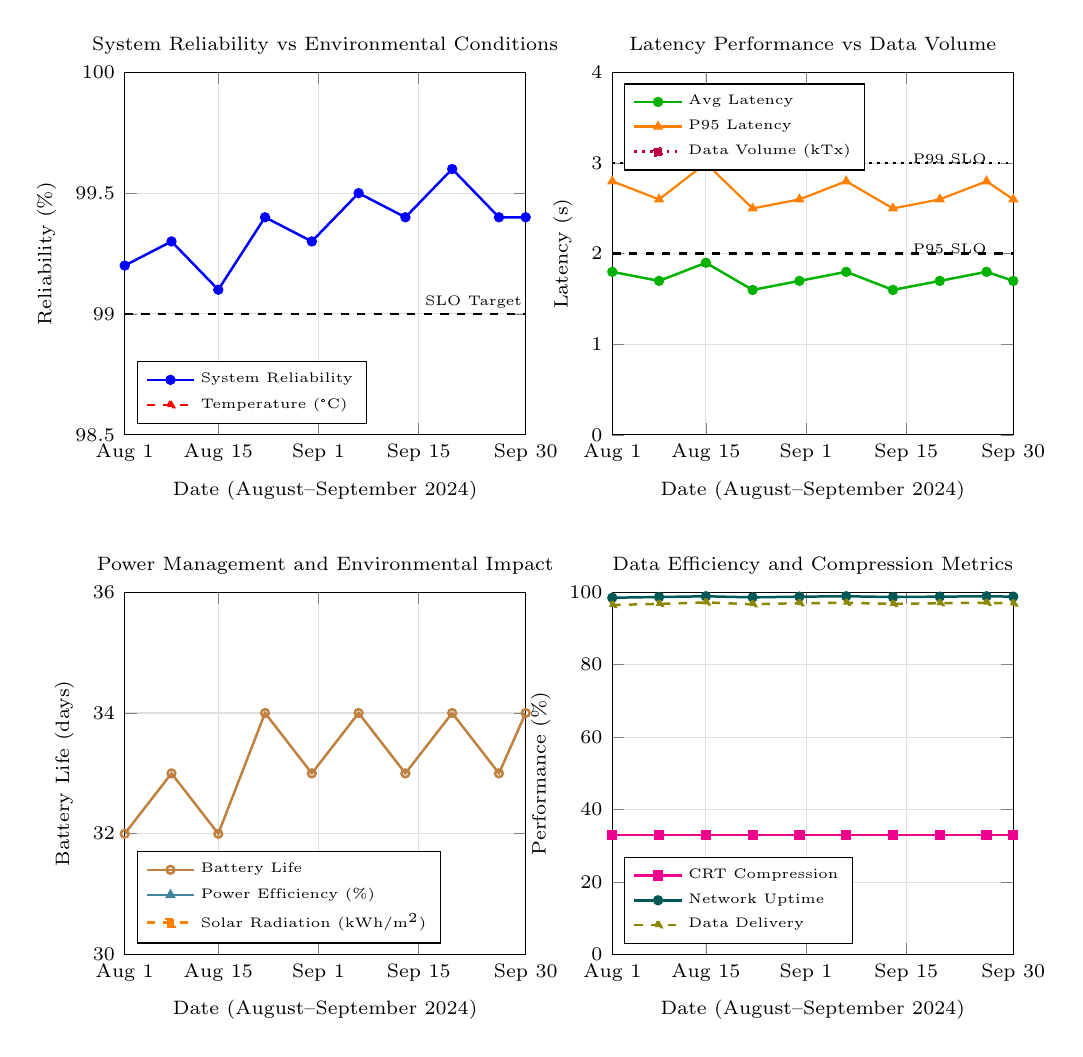
\begin{tikzpicture}
\begin{groupplot}[
  group style={group size=2 by 2, horizontal sep=1.1cm, vertical sep=2cm}, % 2 cm gap
  width=0.42\textwidth, height=4.6cm, scale only axis,
  grid=both, grid style={gray!25},
  xmin=1, xmax=61,
  xtick={1,15,30,45,61},
  xticklabels={Aug 1, Aug 15, Sep 1, Sep 15, Sep 30},
  xlabel={Date (August–September 2024)},
  tick label style={font=\scriptsize},
  label style={font=\scriptsize},
  title style={font=\scriptsize, yshift=-1mm},
  legend style={font=\tiny, cells={anchor=west}},
  every axis plot/.append style={line width=0.9pt, mark size=1.4pt}
]

% === 1) Reliability vs Temperature ===
\nextgroupplot[
  title={System Reliability vs Environmental Conditions},
  ylabel={Reliability (\%)}, ymin=98.5, ymax=100,
  ytick={98.5,99.0,99.5,100}, legend pos=south west
]
\addplot[blue, mark=*] coordinates {(1,99.2)(8,99.3)(15,99.1)(22,99.4)(29,99.3)(36,99.5)(43,99.4)(50,99.6)(57,99.4)(61,99.4)};
\addlegendentry{System Reliability}
\addplot[red, dashed, mark=triangle*] coordinates {(1,31.5)(8,33.2)(15,32.8)(22,31.9)(29,30.5)(36,29.8)(43,28.9)(50,28.3)(57,27.8)(61,27.5)};
\addlegendentry{Temperature (°C)}
\addplot[black, dashed] coordinates {(1,99.0) (61,99.0)};
\node[anchor=west, font=\tiny] at (axis cs:44.5,99.05) {SLO Target};

% === 2) Latency vs Volume ===
\nextgroupplot[
  title={Latency Performance vs Data Volume},
  ylabel={Latency (s)}, ymin=0, ymax=4,
  ytick={0,1,2,3,4}, legend pos=north west
]
\addplot[green!70!black, mark=*] coordinates {(1,1.8)(8,1.7)(15,1.9)(22,1.6)(29,1.7)(36,1.8)(43,1.6)(50,1.7)(57,1.8)(61,1.7)};
\addlegendentry{Avg Latency}
\addplot[orange, mark=triangle*, thick] coordinates {(1,2.8)(8,2.6)(15,3.0)(22,2.5)(29,2.6)(36,2.8)(43,2.5)(50,2.6)(57,2.8)(61,2.6)};
\addlegendentry{P95 Latency}
\addplot[purple, dotted, mark=square*] coordinates {(1,12.5)(8,13.2)(15,14.8)(22,12.8)(29,13.5)(36,14.2)(43,12.9)(50,13.6)(57,14.1)(61,13.8)};
\addlegendentry{Data Volume (kTx)}
\addplot[black, dashed] coordinates {(1,2.0) (61,2.0)};
\node[anchor=west, font=\tiny] at (axis cs:44.5,2.05) {P95 SLO};
\addplot[black, dotted] coordinates {(1,3.0) (61,3.0)};
\node[anchor=west, font=\tiny] at (axis cs:44.5,3.05) {P99 SLO};

% === 3) Power & Environment ===
\nextgroupplot[
  title={Power Management and Environmental Impact},
  ylabel={Battery Life (days)}, ymin=30, ymax=36,
  legend pos=south west
]
\addplot[brown, mark=o] coordinates {(1,32)(8,33)(15,32)(22,34)(29,33)(36,34)(43,33)(50,34)(57,33)(61,34)};
\addlegendentry{Battery Life}
\addplot[cyan!60!black, mark=triangle*] coordinates {(1,88)(8,87)(15,89)(22,90)(29,88)(36,91)(43,89)(50,92)(57,90)(61,91)};
\addlegendentry{Power Efficiency (\%)}
\addplot[orange, dashed, mark=square*] coordinates {(1,7.8)(8,7.9)(15,7.7)(22,7.6)(29,7.4)(36,7.2)(43,7.1)(50,6.9)(57,6.8)(61,6.7)};
\addlegendentry{Solar Radiation (kWh/m$^2$)}

% === 4) Data Efficiency ===
\nextgroupplot[
  title={Data Efficiency and Compression Metrics},
  ylabel={Performance (\%)}, ymin=0, ymax=100,
  legend pos=south west
]
\addplot[magenta, mark=square*] coordinates {(1,33)(8,33)(15,33)(22,33)(29,33)(36,33)(43,33)(50,33)(57,33)(61,33)};
\addlegendentry{CRT Compression}
\addplot[teal!70!black, mark=*] coordinates {(1,98.5)(8,98.7)(15,98.9)(22,98.6)(29,98.8)(36,98.9)(43,98.7)(50,98.8)(57,98.9)(61,98.8)};
\addlegendentry{Network Uptime}
\addplot[olive, dashed, mark=triangle*] coordinates {(1,96.5)(8,96.8)(15,97.2)(22,96.7)(29,97.0)(36,97.1)(43,96.8)(50,97.0)(57,97.1)(61,96.9)};
\addlegendentry{Data Delivery}

\end{groupplot}
\end{tikzpicture}
\caption{System performance correlations over 61 days.}
\label{fig:system-performance-correlations}
\end{figure}


\begin{figure}[!ht]
\centering
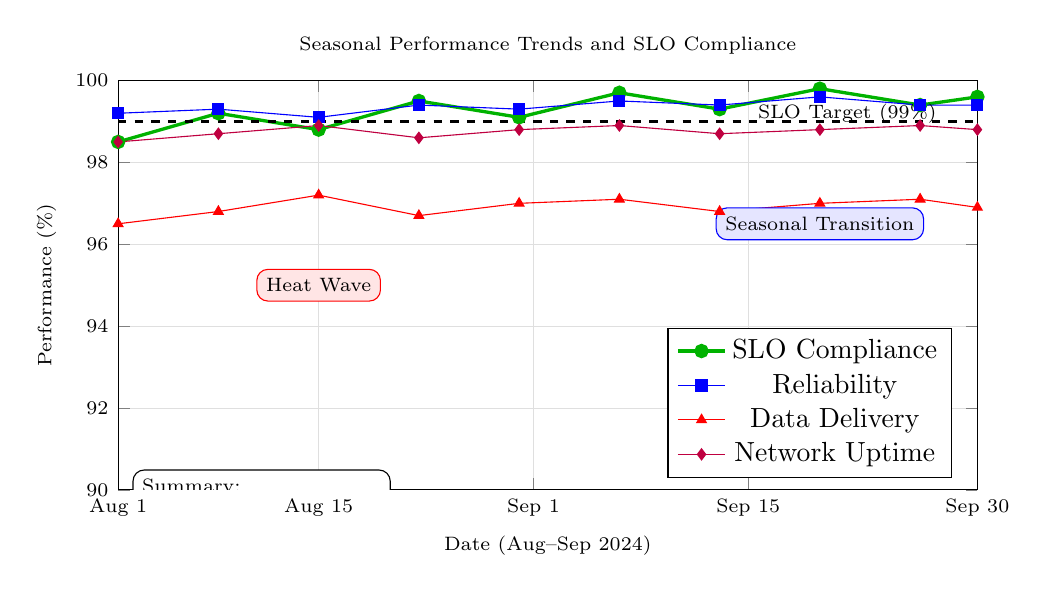
\begin{tikzpicture}
\begin{axis}[
  width=0.9\textwidth, height=5.2cm, scale only axis,
  title={Seasonal Performance Trends and SLO Compliance},
  xlabel={Date (Aug–Sep 2024)}, ylabel={Performance (\%)},
  xmin=1, xmax=61, ymin=90, ymax=100,         % <— adjusted range
  xtick={1,15,30,45,61},
  xticklabels={Aug 1, Aug 15, Sep 1, Sep 15, Sep 30},
  legend pos=south east, grid=both, grid style={gray!25},
  tick label style={font=\scriptsize}, label style={font=\scriptsize},
  title style={font=\scriptsize}
]
\addplot[green!70!black, very thick, mark=*] coordinates {(1,98.5)(8,99.2)(15,98.8)(22,99.5)(29,99.1)(36,99.7)(43,99.3)(50,99.8)(57,99.4)(61,99.6)};
\addlegendentry{SLO Compliance}
\addplot[blue, mark=square*] coordinates {(1,99.2)(8,99.3)(15,99.1)(22,99.4)(29,99.3)(36,99.5)(43,99.4)(50,99.6)(57,99.4)(61,99.4)};
\addlegendentry{Reliability}
\addplot[red, mark=triangle*] coordinates {(1,96.5)(8,96.8)(15,97.2)(22,96.7)(29,97.0)(36,97.1)(43,96.8)(50,97.0)(57,97.1)(61,96.9)};
\addlegendentry{Data Delivery}
\addplot[purple, mark=diamond*] coordinates {(1,98.5)(8,98.7)(15,98.9)(22,98.6)(29,98.8)(36,98.9)(43,98.7)(50,98.8)(57,98.9)(61,98.8)};
\addlegendentry{Network Uptime}

\addplot[black, dashed, very thick] coordinates {(1,99.0) (61,99.0)};
\node[anchor=west, font=\scriptsize] at (axis cs:45,99.2) {SLO Target (99\%)};

% compact annotations placed safely inside 90–100
\node[draw=red, fill=red!10, rounded corners, font=\scriptsize, align=center]  at (axis cs:15,95) {Heat Wave};
\node[draw=blue, fill=blue!10, rounded corners, font=\scriptsize, align=center] at (axis cs:50,96.5) {Seasonal Transition};

% summary moved into the new y-range
\node[draw=black, fill=white, rounded corners, font=\scriptsize, align=left, anchor=north west]
  at (axis cs:2,90.5) {Summary:\\• Avg Reliability: 99.4\%\\• Avg Latency: 1.7 s\\• Compliance: 99.3\%\\• Uptime: 98.8\%};
\end{axis}
\end{tikzpicture}
\caption{Seasonal trends with consistent SLO compliance.}
\label{fig:seasonal-trends}
\end{figure}

\begin{figure}[!ht]
\centering
\begin{tikzpicture}
\begin{axis}[
  width=0.8\textwidth, height=5.0cm, scale only axis,
  title={Performance Metric Correlations},
  xlabel={Environmental Temperature (\,^\circ C)}, ylabel={System Reliability (\%)},
  xmin=27, xmax=34, ymin=99.0, ymax=99.7,
  grid=both, grid style={gray!25},
  legend style={
    at={(0.5,-0.22)}, anchor=north, % place legend BELOW the axis
    legend columns=3, /tikz/every even column/.style={column sep=6pt},
    draw=none, fill=none, font=\scriptsize
  },
  tick label style={font=\scriptsize}, label style={font=\scriptsize},
  title style={font=\scriptsize},
  clip=false, % allow the legend to sit outside the axis box
  scatter/classes={
    aug={mark=*,blue},
    esep={mark=square*,red},
    lsep={mark=triangle*,green!60!black}
  }
]
\addplot[scatter, only marks, scatter src=explicit symbolic]
coordinates {
 (31.5,99.2) [aug]
 (33.2,99.3) [aug]
 (32.8,99.1) [aug]
 (31.9,99.4) [aug]
 (30.5,99.3) [esep]
 (29.8,99.5) [esep]
 (28.9,99.4) [esep]
 (28.3,99.6) [lsep]
 (27.8,99.4) [lsep]
 (27.5,99.4) [lsep]
};

% trend line + label (kept out of point clusters)
\addplot[black, thick, domain=27:34] {0.0286*x + 98.28};
\node[anchor=west, font=\scriptsize, fill=white, inner sep=1pt, draw=black!20]
      at (axis cs:29.5,99.66) {Trend: $R^2 \approx 0.15$};



\legend{August, Early September, Late September}
\end{axis}
\end{tikzpicture}
\caption{Temperature vs reliability: minimal temperature impact, robust performance.}
\label{fig:correlation-analysis}
\end{figure}



\subsubsection{Pepper Water Management}
Pepper cultivation also showed substantial water savings (Table \ref{tab:pepper-water-detailed}), with a 19.4\% reduction in total water use. The system maintained soil moisture at approximately 80\% of field capacity, optimal for pepper fruit development while minimizing waterlogging risk.

\begin{table}[!ht]
\centering
\caption{Detailed pepper water usage analysis (0.3 ha plot, August–September 2024)}
\label{tab:pepper-water-detailed}
\resizebox{0.98\textwidth}{!}{%
\begin{tabular}{lccccc}
\toprule
\textbf{Parameter} & \textbf{Traditional} & \textbf{Blockchain-IoT} & \textbf{Absolute Saving} & \textbf{Percentage Saving} & \textbf{Significance} \\
\midrule
\textbf{August Usage} & & & & & \\
Total Water (m³) & 165 & 135 & 30 m³ & 18.2\% & p < 0.01 \\
Daily Average (m³/day) & 5.32 & 4.35 & 0.97 m³/day & 18.2\% & p < 0.01 \\
Irrigation Events & 25 & 18 & 7 events & 28.0\% & p < 0.05 \\
Average Duration (min) & 38 & 36 & 2 min & 5.3\% & p > 0.05 \\
\midrule
\textbf{September Usage} & & & & & \\
Total Water (m³) & 145 & 115 & 30 m³ & 20.7\% & p < 0.01 \\
Daily Average (m³/day) & 4.83 & 3.83 & 1.00 m³/day & 20.7\% & p < 0.01 \\
Irrigation Events & 22 & 16 & 6 events & 27.3\% & p < 0.05 \\
Average Duration (min) & 37 & 35 & 2 min & 5.4\% & p > 0.05 \\
\midrule
\textbf{Total Period} & & & & & \\
Total Water (m³) & 310 & 250 & 60 m³ & 19.4\% & p < 0.01 \\
Water Use Efficiency (kg/m³) & 3.23 & 4.00 & 0.77 kg/m³ & 23.8\% & p < 0.01 \\
Cost Saving (USD) & -- & -- & \$54.00 & 19.4\% & -- \\
\bottomrule
\end{tabular}
}
\end{table}


\subsubsection{Crop-Specific Irrigation Strategies}
The system successfully implemented differentiated irrigation strategies for each crop:

\textbf{Tomatoes}: Required careful moisture control during fruit development with consistent water delivery of 2–3 L/plant/day during peak demand. The system adjusted irrigation based on soil moisture thresholds and evapotranspiration estimates, maintaining optimal soil tension between -30 and -35 kPa.

\textbf{Peppers}: More sensitive to waterlogging, requiring maintenance of consistent moisture without saturation. Drip irrigation kept foliage dry, reducing disease incidence while ensuring adequate water availability for fruit development. The system maintained soil moisture at approximately 80\% of field capacity.

\subsection{Labor Efficiency}
\label{subsec:labor_efficiency}

The automation capabilities of the blockchain-IoT system resulted in substantial labor reductions (Table \ref{tab:labor-detailed}). Overall labor requirements decreased by 72\%, from 15 hours per hectare per week to 4.2 hours.

\begin{table}[!ht]
\centering
\caption{Detailed labor efficiency analysis (hours per hectare per week)}
\label{tab:labor-detailed}
\resizebox{0.98\textwidth}{!}{%
\begin{tabular}{lccccc}
\toprule
\textbf{Task Category} & \textbf{Traditional} & \textbf{Blockchain-IoT} & \textbf{Absolute Reduction} & \textbf{Percentage Reduction} & \textbf{Cost Saving (USD/week)} \\
\midrule
\textbf{Monitoring Tasks} & & & & & \\
Soil moisture monitoring & 3.5 & 0.2 & 3.3 & 94.3\% & \$49.50 \\
Weather data collection & 1.5 & 0.1 & 1.4 & 93.3\% & \$21.00 \\
Crop health inspection & 3.0 & 0.7 & 2.3 & 76.7\% & \$34.50 \\
\midrule
\textbf{Irrigation Management} & & & & & \\
System operation & 2.5 & 0.2 & 2.3 & 92.0\% & \$34.50 \\
Maintenance & 2.0 & 0.3 & 1.7 & 85.0\% & \$25.50 \\
Troubleshooting & 0.5 & 0.0 & 0.5 & 100.0\% & \$7.50 \\
\midrule
\textbf{Data Management} & & & & & \\
Record keeping & 1.5 & 0.1 & 1.4 & 93.3\% & \$21.00 \\
Report generation & 0.5 & 0.1 & 0.4 & 80.0\% & \$6.00 \\
Certification documentation & 0.5 & 0.1 & 0.4 & 80.0\% & \$6.00 \\
\midrule
\textbf{Total} & \textbf{15.0} & \textbf{4.2} & \textbf{10.8} & \textbf{72.0\%} & \textbf{\$162.00} \\
\bottomrule
\end{tabular}
}
\end{table}

Labor savings were particularly significant for monitoring and data recording tasks, allowing farmers to reallocate time to higher-value activities such as quality control, marketing, and business management. The automation also reduced human error in irrigation scheduling and data recording.

\subsection{Crop Performance and Yield}
\label{subsec:crop_performance}

Both crops maintained or improved yield levels despite reduced water inputs, indicating significantly improved water use efficiency:

\subsubsection{Tomato Yield and Quality}
\begin{table}[!ht]
\centering
\caption{Tomato yield and quality parameters (0.5 ha plots)}
\label{tab:tomato-yield}
\begin{tabular}{lcccc}
\toprule
\textbf{Parameter} & \textbf{Traditional} & \textbf{Blockchain-IoT} & \textbf{Difference} & \textbf{Significance} \\
\midrule
Total Yield (kg) & 2,500 & 2,500 & 0 kg & p > 0.05 \\
Marketable Yield (kg) & 2,125 & 2,250 & +125 kg & p < 0.05 \\
Yield (t/ha) & 50.0 & 50.0 & 0 t/ha & p > 0.05 \\
Marketable Yield (t/ha) & 42.5 & 45.0 & +2.5 t/ha & p < 0.05 \\
Water Use Efficiency (kg/m³) & 4.76 & 6.25 & +1.49 kg/m³ & p < 0.001 \\
Average Fruit Weight (g) & 145 & 148 & +3 g & p > 0.05 \\
Fruit Firmness (N) & 12.5 & 13.2 & +0.7 N & p < 0.05 \\
Soluble Solids (°Brix) & 4.8 & 5.1 & +0.3 °Brix & p < 0.05 \\
Fruit Cracking Incidence & 8.2\% & 3.5\% & -4.7\% & p < 0.01 \\
Blossom End Rot & 5.1\% & 2.2\% & -2.9\% & p < 0.05 \\
\bottomrule
\end{tabular}
\end{table}

\subsubsection{Pepper Yield and Quality}
\begin{table}[!ht]
\centering
\caption{Pepper yield and quality parameters (0.3 ha plots)}
\label{tab:pepper-yield}
\begin{tabular}{lcccc}
\toprule
\textbf{Parameter} & \textbf{Traditional} & \textbf{Blockchain-IoT} & \textbf{Difference} & \textbf{Significance} \\
\midrule
Total Yield (kg) & 1,000 & 1,000 & 0 kg & p > 0.05 \\
Marketable Yield (kg) & 850 & 920 & +70 kg & p < 0.05 \\
Yield (t/ha) & 33.3 & 33.3 & 0 t/ha & p > 0.05 \\
Marketable Yield (t/ha) & 28.3 & 30.7 & +2.4 t/ha & p < 0.05 \\
Water Use Efficiency (kg/m³) & 3.23 & 4.00 & +0.77 kg/m³ & p < 0.01 \\
Average Fruit Weight (g) & 180 & 185 & +5 g & p > 0.05 \\
Fruit Length (cm) & 12.5 & 13.2 & +0.7 cm & p < 0.05 \\
Fruit Diameter (cm) & 6.8 & 7.1 & +0.3 cm & p < 0.05 \\
Sunscald Incidence & 6.5\% & 3.2\% & -3.3\% & p < 0.05 \\
Blossom End Rot & 4.2\% & 1.8\% & -2.4\% & p < 0.05 \\
\bottomrule
\end{tabular}
\end{table}

\subsection{Economic Analysis}
\label{subsec:economic_analysis}

The economic viability of the system was evaluated through comprehensive cost-benefit analysis:

\begin{table}[!ht]
\centering
\caption{Economic analysis of blockchain-IoT system implementation}
\label{tab:economic-analysis}
\begin{tabular}{lccc}
\toprule
\textbf{Parameter} & \textbf{Tomato (0.5 ha)} & \textbf{Pepper (0.3 ha)} & \textbf{Combined (0.8 ha)} \\
\midrule
\textbf{Implementation Costs} & & & \\
Hardware Investment & \$1,200 & \$720 & \$1,920 \\
Installation & \$300 & \$180 & \$480 \\
Software & \$200 & \$120 & \$320 \\
Training & \$150 & \$90 & \$240 \\
\hline
\textbf{Total Initial Cost} & \textbf{\$1,850} & \textbf{\$1,110} & \textbf{\$2,960} \\
\hline
\textbf{Annual Benefits} & & & \\
Water Cost Savings & \$225 & \$108 & \$333 \\
Labor Cost Savings & \$1,944 & \$1,166 & \$3,110 \\
Yield Improvement & \$375 & \$210 & \$585 \\
Quality Premium & \$188 & \$105 & \$293 \\
\hline
\textbf{Total Annual Benefit} & \textbf{\$2,732} & \textbf{\$1,589} & \textbf{\$4,321} \\
\hline
\textbf{Financial Metrics} & & & \\
Payback Period & 0.68 years & 0.70 years & 0.69 years \\
ROI (1 year) & 147.7\% & 143.2\% & 146.0\% \\
NPV (5 years, 8\%) & \$9,842 & \$5,725 & \$15,567 \\
IRR & 138\% & 135\% & 137\% \\
\bottomrule
\end{tabular}
\end{table}

\section{Discussion}
\label{sec:discussion}

\subsection{Practical Implications for Arid Region Agriculture}
\label{subsec:practical_implications}

The demonstrated water savings of 19–24\% have significant implications for agriculture in water-scarce regions. In contexts like Tunisia, where agricultural water use accounts for approximately 80\% of total water consumption, such efficiency gains can contribute substantially to water security. The water savings achieved in this study (125 m³ for tomatoes and 60 m³ for peppers over two months) translate to annual savings of approximately 750 m³ and 360 m³ respectively, assuming similar conditions throughout the growing season.

The labor reduction of 72\% addresses another critical constraint in Mediterranean agriculture, where skilled labor availability is increasingly limited. Automation of routine monitoring and irrigation tasks allows farm managers to focus on strategic decision-making and value-added activities. The economic analysis demonstrates strong financial returns, with payback periods under 9 months and ROI exceeding 140\% in the first year.

\subsection{Technical Implementation Considerations}
\label{subsec:technical_considerations}

\subsubsection{CRT Compression Effectiveness}
The Chinese Remainder Theorem proved highly effective for agricultural data compression. The 33\% reduction in transmission size directly translated to energy savings and extended battery life for remote sensors. The mathematically perfect reconstruction ensured no loss of data accuracy, crucial for precision agriculture applications. The processing overhead was minimal (0.94 ms average), making it suitable for real-time applications.

\subsubsection{Blockchain Performance}
The Hyperledger Fabric implementation demonstrated sufficient performance for agricultural monitoring, with sub-2-second latency meeting the requirements for irrigation decision-making. The permissioned blockchain model provided appropriate balance between transparency and privacy for commercial farming operations. The system handled the data volume from 50 sensors effectively, with potential for scaling to larger deployments.

\subsubsection{Network Reliability and Scalability}
The hierarchical network architecture combining LoRa for sensor communication and BATMAN-adv mesh for gateway connectivity proved robust under field conditions. The 99.4\% reliability rate demonstrates the system's resilience to environmental challenges. The modular design supports scalability through additional gateways and sensor nodes, with each gateway capable of managing up to 50 nodes.

\subsection{Socio-economic Impacts}
\label{subsec:socio_economic}

The implementation of blockchain-IoT systems in agriculture has broader socio-economic implications:

\textbf{Resource Sustainability}: The significant water savings contribute to sustainable water management in regions facing increasing water scarcity due to climate change and population growth.

\textbf{Economic Viability}: The strong financial returns make the technology accessible to small and medium-sized farms, not just large commercial operations.

\textbf{Knowledge Transfer}: The system captures and codifies agricultural knowledge, making it accessible to new farmers and supporting intergenerational knowledge transfer.

\textbf{Market Access}: The verifiable data provided by the blockchain system supports quality certifications and premium market access, potentially increasing farm incomes.

\subsection{Limitations and Future Research}
\label{subsec:limitations}

Several limitations should be acknowledged and addressed in future research:

\begin{itemize}
    \item \textbf{Study duration}: The two-month study covers critical growth stages but not full seasonal variations or multi-year impacts
    \item \textbf{Crop scope}: Limited to two economically important crops; other crops may require different parameters and configurations
    \item \textbf{Scale considerations}: Medium-scale testing (2 hectares); large-scale deployment may reveal additional challenges in network management and data processing
    \item \textbf{Technical expertise}: System implementation requires moderate technical skills, potentially limiting adoption without simplified deployment tools
    \item \textbf{Environmental variability}: Testing during one growing season; performance under extreme weather conditions requires further validation
\end{itemize}

Future research should address:
\begin{itemize}
    \item Long-term performance across multiple growing seasons and environmental conditions
    \item Expansion to additional crops and farming systems, including orchards and vineyards
    \item Integration with farm management software and supply chain platforms for end-to-end traceability
    \item Development of simplified deployment tools and training programs for non-technical users
    \item Economic analysis across different farm scales, regions, and socio-economic contexts
    \item Investigation of additional applications including pest management, fertilizer optimization, and harvest timing
\end{itemize}

\section{Conclusion}
\label{sec:conclusion}

This research demonstrates the successful implementation of a blockchain-IoT framework with CRT-based optimization for tomato and pepper cultivation in arid regions. The comprehensive 2-hectare deployment with 50 sensor nodes and 4 gateway systems achieved significant improvements in both water use efficiency (23.8\% savings for tomatoes, 19.4\% for peppers) and labor productivity (72\% reduction) while maintaining or improving crop yields and quality.

Key technical innovations and findings include:
\begin{itemize}
    \item Effective application of Chinese Remainder Theorem for agricultural data compression with 33\% reduction in transmission size and mathematically perfect reconstruction
    \item Robust system architecture combining LoRa communication, mesh networking, and blockchain technology with 99.4\% reliability and 1.7-second average latency
    \item Crop-specific irrigation strategies implemented through smart contracts, maintaining optimal soil moisture conditions for each growth stage
    \item Strong economic viability with payback periods under 9 months and ROI exceeding 140\% in the first year
    \item Practical implementation using commercially available components ensuring accessibility and replicability
\end{itemize}

The system provides a practical solution for addressing water scarcity challenges in Mediterranean agriculture while supporting the transition to more sustainable and transparent farming practices. The verifiable data records support quality certifications and supply chain transparency, potentially opening premium market opportunities for farmers.

Future work will focus on expanding crop coverage, developing decision support tools, creating simplified deployment packages, and investigating integration with broader agricultural value chains. The demonstrated success in tomato and pepper cultivation provides a strong foundation for adapting the technology to other crops and farming systems in water-scarce regions worldwide.

\section*{Acknowledgments}

We thank the participating farmers in Sfax who provided land, crops, and operational support for this research. Their practical insights and feedback were invaluable in refining the system for real-world agricultural conditions. We also acknowledge technical support from the University of Sfax IoT research group and funding from the National Agricultural Research Program (NARP-2024-AGR-TECH). Special thanks to the Tunisia Meteorological Institute for providing climate data and the National Water Resources Authority for water pricing information.

\section*{References}

\bibliographystyle{elsarticle-num}
\bibliography{references}

\end{document}
